

%\documentclass[aip,graphicx]{revtex4-1}
\documentclass[aip,jap, amsmath,amssymb,reprint]{revtex4-1}

\usepackage{graphicx}% Include figure files
\usepackage{dcolumn}% Align table columns on decimal point
\usepackage{bm}% bold math
%\usepackage[mathlines]{lineno}% Enable numbering of text and display math
%\linenumbers\relax % Commence numbering lines
%\draft % marks overfull lines with a black rule on the right
\usepackage{multirow}

\begin{document}

\preprint{AIP/123-QED}

%\title{Irradiation influence on  acousto--defect interaction in silicon $n^+$-$p$--structure}
\title{Acousto--defect interaction in irradiated and non--irradiated silicon $n^+$--$p$--structure}
\author{O.~Ya. Olikh}
\email{olikh@univ.kiev.ua}


\author{A.~M. Gorb}


\author{R.~G. Chupryna}

\author{O.~V. Pristay--Fenenkov}%


\affiliation{Faculty of Physics, Taras Shevchenko National University of Kyiv, Kyiv 01601, Ukraine}%Lines break automatically or can be forced with \\



\date{\today}

\begin{abstract}
The experimental investigation of ultrasound influence on the electrical characteristics of silicon $n^+$--$p$--structure has been carried out.
The effects of reactor neutrons and $^{60}$Co gamma radiation on ultrasound influence were studied.
It has been found out that the ultrasound loading leads to reversible change of shunt resistance, carrier lifetime in both space charge and quasi--neutral regions, ideality factor.
Acoustically induced alteration of last two parameters depends on irradiation considerably.
The models of coupled defect level recombination, Shockley--Read--Hall recombination, and dislocation--induced impedance were used to describe findings.
It has been shown that the observed phenomena can deal with the increase of distance between coupled defects as well as an extension of carrier capture coefficient of complex point defect and dislocation.
It has been shown that divacancy and pair vacancy--interstitial oxygen are effectively modified by ultrasound in contrast to complex interstitial carbon--interstitial oxygen.
\end{abstract}

%\pacs{73.30.+y}
\keywords{acousto--defect interaction, silicon, irradiation}

\maketitle %\maketitle must follow title, authors, abstract and \pacs

\section{Introduction}
It has been shown experimentally that ultrasound (US) can effectively interact with defects.
US as defect engineering tool has some advantages:
(i)~locality of the action due to the predominant absorption in regions of deviation in the lattice periodicity;
(ii)~selectivity of the influence, which is achieved by variation of acoustic wave (AW) polarization and type;
(iii)~possibility of resonance transformation in the defect system due to the oscillation nature of action;
(iv)~capability of reversible effect in the case of low intensity AW.

In the case of piezoelectric semiconductors, the acousto--defect interaction (ADI) is determined mainly by electric field, which accompanies the vibration wave propagation.
This effect is expected and something related to acousto--electric phenomena.
But US influence on defect system is also observed in non--piezoelectric crystals like silicon, which is microelectronic dominant material.
Thus it was experimentally observed in silicon structures, that US
caused an atomic diffusion, \cite{Roman:2010JAP,Roman:2007APL}
transformed a native and an impurity defect, \cite{Ostapenko1994,Korotchenkov1995,Olikh2009Sem,Ostapenko1995,Ostrovskii2001}
modified  interior surface states,\cite{UST:Medvid,Zaver:2008,Mirsagatov}
created new defect. \cite{Savkina2015,Virot}
Defects are known to determine a most of semiconductor device properties.
And exactly the ADI is a reason of variation of a tunneling, \cite{Olikh2016JSem,Olikh2011Sem} a generation--recombination \cite{Davletova2009,Davletova2008,YOlikh2005} and  a thermionic emission \cite{OlikhJAP,Olikh:Ultras} current in silicon barrier structures.

The main mechanisms of elastic vibration--defect interaction in non-piezoelectric crystals are considered to be
the  change  of  population  of  impurity  oscillator  levels,  \cite{Pavlovich}
the displacement of impurity atoms with respect to their surroundings, \cite{Korotchenkov1995,MirzadeJAP2011,PeleshchakUJF2016}
the decreasing of the diffusion activation  energy, \cite{Krevchik}
the local temperature increase by point defect clusters, \cite{MirzadeJAP2005}
the US absorption by dislocation. \cite{Davletova2008,OstrovKor92,Olikh:Ultras2016}
However to the best of our knowledge, the complete ADI theory in silicon is absent.
One of a top--ranked cause
%of  this situation
is a lack of experimental works, which have focused on investigation of acoustically induced (AI) effects.

Not all silicon defects are acoustically active and subjected to modification under US action.
The ADI efficiency depends on the defect type and structure. \cite{UST:Medvid}
Thus, the force acting on the point defect during US loading (USL) is determined by the relaxation of the defect volume\cite{MirzadeJAP2011,PeleshchakUJF2016}.
The irradiation is most widespread and studied method of semiconductor defects alteration.
On the one hand, the high--power US treatment is shown\cite{YOlikh2007TPL,Parchinskii2006,Gorb2010,Podolian2012} to lead to residual changes of the irradiated silicon structure properties.
This effect deals with AI annealing of radiation defects (RDs).
On the other hand, irradiation can be a reason of reversible AI phenomenon initiation, \cite{YOlikh2006TPL,YOlikhTPL2011} which is caused by formation of acoustically active RDs.
Unfortunately, there have only a few reports on acoustically driven phenomenon in irradiated silicon structures.


Our goal is to investigate experimentally the AI electrical characteristic variation, which takes place in non--irradiated and irradiated $n^+$--$p$--Si structures.
Irradiation was carried by reactor neutrons and a $^{60}$Co--gamma source.
It is expected that $\gamma$--rays introduce
%vacancy--impurity point defects (
VO$_i$ complex predominantly,
%)
\cite{NIEL:Jafari,Gamma:Prabhakara,NIEL:Moll}
whereas neutrons create vacancy clusters, \cite{Rew:Srour,Pintilie} disordered regions \cite{Neutron:Arutyunov} and C$_i$O$_i$ complex  \cite{NIEL:Moll,neutron:Londos} mainly.
This work represents distinction of AI effects in silicon structures with different RDs.
The used US intensity was not very high
%($<0.5$~W/cm$^2$)
to avoid the irreversible defect subsystem modification,
which can deal with a new defect creation, a RDs annealing or a long distance (a many interatomic distance) diffusion.
As a result, the characteristic full recovery was observed after the stop of an AW propagation.
The models of coupled defect level recombination, \cite{CDLR:JAP1995,CDLR:JAP} Shockley--Read--Hall (SRH) recombination, and dislocation--induced impedance \cite{Rsh:Gopal2003,Rsh:Gopal2004} were used to describe the processes in the space charge region (SCR),  in the diode base, and shunt resistance, respectively.
The interaction of defects with an AW strain field \cite{MirzadeJAP2011,PeleshchakUJF2016} was recruited to explain the observed AI phenomena.
The investigation would provide not only better ADI understanding but could also facilitate the development of acoustically controlled devices or radiation sensors.



\section{Experimental and calculation details}

The 2~inch (300~$\mu$m thick) p--type boron doped, $<$111$>$ orientation, Czochralski silicon wafer having resistivity of 10~$\Omega\cdot$cm was used for fabrication of  $n^+$-$p$--Si structure.
The n$^+$ emitter with carrier concentration of about $10^{19}$~cm$^{-3}$ and thickness of 0.5~$\mu$m was formed by phosphorus implantation.
Aluminium front and rear electrodes were deposited by screen printing before rapid annealing.
%Then wafer surface was passivated by Al$_2$O$_3$ film and further capped by TiO$_x$ as antireflective coating.
%Finally the aluminium front (metal grid) and rear (solid contact) electrodes were deposited by screen printing before rapid annealing.
Samples with area of about $2$~cm$^{2}$ were cut from the central part of the wafer and used in experiment.
Samples were irradiated by reactor neutrons or by $^{60}$Co $\gamma$--rays.
Doses $D$, fluences $\Psi$, and sample labels are listed in Table~\ref{tabSample}.
Data \cite{NIEL:Akkerman,Brauning} were used to determine $D$ and $\Psi$ correlation.
The non--ionizing energy losses (NIEL) for neutron and $\gamma$--$^{60}$Co are shown in Table~\ref{tabSample} too.
As displacement damage effect is characterized by $(\Psi\cdot \mbox{NIEL})$,
the similar damage is expected in investigated samples.
To avoid an impact of  long--term annealing, which is typical to neutron damaged structure especially, \cite{NIEL:Moll,Rew:Srour} irradiated samples have been stored  for  5 years  at  room  temperature before measuring.

\begin{table}
\caption{\label{tabSample}The sample irradiation parameters.
}
\begin{ruledtabular}
\begin{tabular}{cccccc}
%\multirow{2}{*}{Sample} &Irradiation&$D$&$\Psi$ &NIEL (Ref.~\onlinecite{NIEL:Akkerman})& $\Psi$ $\times$NIEL  \\
\multirow{2}{*}{Sample} &Irradiation&$D$&$\Psi$ &NIEL\footnote{Ref.~\onlinecite{NIEL:Akkerman}.}& $\Psi$ $\times$NIEL  \\
&type& (rad)& (cm$^{-2}$)&(MeV~cm$^2$/g)& (MeV/g) \\
\hline
iSC&non&0&0&---&0\\
nSC&neutron&4.5$\cdot$10$^3$&4$\cdot$10$^{11}$&2.04$\cdot$10$^{-3}$&8.2$\cdot$10$^{8}$\\
g6SC&$\gamma$--$^{60}$Co&1$\cdot$10$^6$&1.6$\cdot$10$^{15}$&1.07$\cdot$10$^{-7}$&1.7$\cdot$10$^{8}$\\
g7SC&$\gamma$--$^{60}$Co&1$\cdot$10$^7$&1.6$\cdot$10$^{16}$&1.07$\cdot$10$^{-7}$&1.7$\cdot$10$^{9}$\\
\end{tabular}
\end{ruledtabular}
\end{table}

%1 sample  was  irradiated  with  neutrons  in  the fluence  of $\Psi_n=4\cdot10^{11}$~n/cm$^2$  and was denoted as nSC.
%2 samples were irradiated  with  $^{60}$Co $\gamma$--rays in the  dose  $D_{\gamma1}=10^6$~rad and $D_{\gamma2}=10^7$~rad and were denoted as g6SC and g7SC respectively.
%The label iSC was used for non--irradiated sample.
%To avoid an impact of  long--term annealing, which are typical to neutron damaged structure especially \cite{NIEL:Moll,Rew:Srour}, irradiated samples were stored  for  5 years  at  room  temperature before measuring.
%According to data \cite{NIEL:Akkerman,Brauning} the neutron dose and gamma fluences can be calculated as $D_n=4.5\cdot10^3$~rad and $\Psi_{\gamma1}=1.6\cdot10^{15}$~$\gamma$/cm$^2$ and $\Psi_{\gamma2}=1.6\cdot10^{16}$~$\gamma$/cm$^2$ respectively.
%The non--ionizing energy losses (NIEL) and lifetime damage--constants ($K_\tau$) for neutron
%differ from $\gamma$--$^{60}$Co ones by four order of magnitude \cite{NIEL:Akkerman,NIEL:Jafari}:
%NIEL$_n=2.04\cdot10^{-3}$~MeV~cm$^2$/g, NIEL$_\gamma=1.07\cdot10^{-7}$~MeV~cm$^2$/g, $K_{\tau,n}=10^{-7}$~cm$^2$/s, $K_{\tau,\gamma}=5\cdot10^{-12}$~cm$^2$/s.
%As $(\Psi_{\gamma1}\cdot K_{\tau,\gamma})<(\Psi_{n}\cdot K_{\tau,n})<(\Psi_{\gamma2}\cdot K_{\tau,\gamma})$,
%neutrons and $\gamma$-rays are expected to produce a similar damage.


The dark forward current--voltage ($I$--$V$) characteristics of the samples both with and without USL were measured over a temperature range 290--340~K.
The temperature was controlled by differential copper--constantan thermocouple.
Some curves are shown in Fig.~\ref{figIV}.


\begin{figure*}
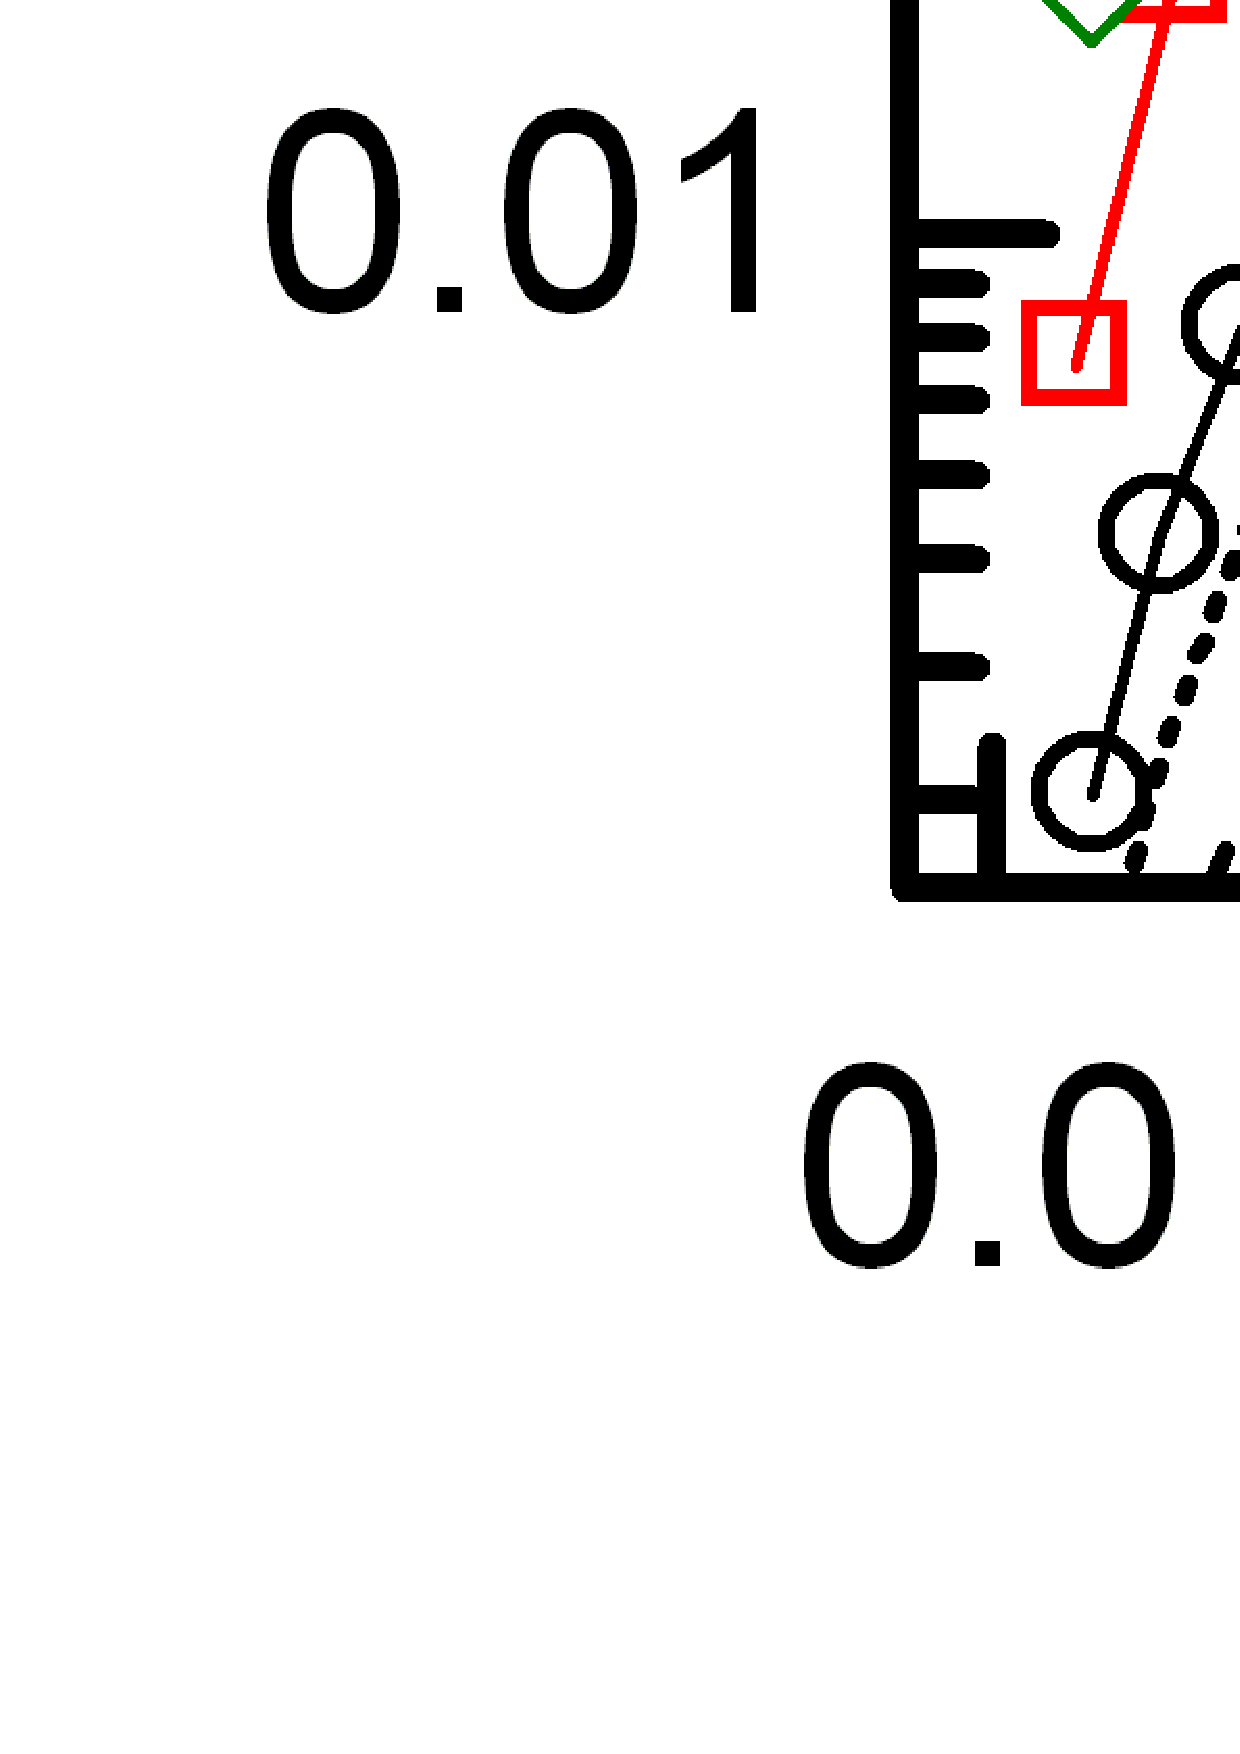
\includegraphics[width=0.7\textwidth]{olikhFig1}%
\caption{\label{figIV}
Dark $I$--$V$ characteristics measured (a) at 306~K for non--irradiated (circles), neutron--irradiated (squares) and gamma--irradiated (diamonds and triangles) structures without USL;
(b) at 301~K (circles) and 341~K (asterisks) with (filled marks, Ui--2) and without (open marks) USL for the iSC.
The marks are the experimental results, the solid lines are the fitted curves using Eqs.~(\ref{eqIV})--(\ref{eqW}).
The dashed, dotted and dot--dashed lines in (a) are the base, SCR and shunt components of iSC current, respectively.
}%
\end{figure*}

The double--diode model of n$^+$--p structure $I$--$V$ characteristic is expressed in the following form:
\begin{eqnarray}
I(V,T)&=&I_{SCR}+I_{base}+I_{sh}\;,\label{eqIV}\\
I_{SCR}&=&\frac{qAn_id}{2\tau_{g}}\left\{\exp \left[\frac{q(V-IR_s)}{n_{\mathrm{id}}kT}\right]-1\right\}\,,\label{eqIscr}\\
I_{base}&=&\frac{qAn_i^2}{p_p}\sqrt{\frac{\mu_nkT}{\tau_n}}\left\{\exp \left[\frac{q(V-IR_s)}{kT}\right]-1\right\},\label{eqIbase}\\
I_{sh}&=&(V-IR_s)/R_{sh}\,,\label{eqIsh}
\end{eqnarray}
where
$I_{SCR}$ reflects the overall SCR recombination,
$I_{base}$ is closely related to recombination in the quasi-neutral region,
$I_{sh}$ is the shunt current,
$A$ is the sample area,
$n_i$ is the intrinsic carrier concentration,
$\tau_{g}$ is the SCR carrier lifetime,
$d$ is the  SCR thickness:
\begin{equation}
\label{eqW}
    d=\sqrt{\frac{2 \varepsilon \varepsilon_0}{q p_p}\left[
     \frac{E_g}{q}-\frac{kT}{q}\ln\!\left(\frac{N_vN_c}{p_pn_n}\right)-\frac{2kT}{q}-V\right]},
\end{equation}
$\varepsilon$ is the permittivity (11.7 for Si),
$p_p$ and $n_n$ are the majority carrier concentration in the $p$-- and $n$--type regions,
$E_g$ is the semiconductor band gap,
$N_c$ and $N_v$ are the effective density of states in the conduction and valence bands;
$n_{\mathrm{id}}$ is the ideality factor,
$R_s$ and $R_{sh}$ are the series and shunt resistances,
$\mu_n$ and $\tau_n$ are the electron (minority carrier) mobility and lifetime in the diode base.


We used Eqs. (\ref{eqIV})--(\ref{eqW}) to fit the experimental data and $\tau_g$, $\tau_n$, $n_{\mathrm{id}}$, $R_{sh}$, and $R_s$ were taken as the  fittings parameters.
The known \cite{ni:Green,Schroder2006,Markvart} temperature dependencies of $n_i$, $E_g$, and $\mu_n$ were used.
The extremely good fit to the experimental data was obtained --- see Fig.~\ref{figIV}.
In particular, the $R_s$ value about 1~$\Omega$ was determined for all samples.


In the USL case, the transverse AWs with frequency of $4.2$~MHz were exited with help of a piezoelectric transducer and were injected in samples from the base side in the [111]--direction.
The US intensities $W_{\mathtt{US}}$, amplitudes of lattice deformation $\xi_{\mathtt{US}}$ and lattice atom
displacement  $u_{\mathtt{US}}$ are listed in Table~\ref{tabUSL}.
It was reported previously \cite{Ostapenko1995,Olikh:Ultras,Ostrovskii2001} that the characteristic time of change in the silicon structure parameters under
the US action  did not exceed $2\cdot10^3$~s.
In order to wait till the AI transitional period the following experimental procedure has been used.
After USL start the sample has been kept at room temperature during 60~min and then the $I$--$V$ measurement and the sample heating were started.
In order to avoid the effect of piezoelectric field on $I$--$V$ characteristics, the piezoelectric transducer has been shielded.


\begin{table}
\caption{\label{tabUSL}The ultrasound loading parameters.
}
\begin{ruledtabular}
\begin{tabular}{ccccc}
Sample&$W_{\mathtt{US}}$ (W/cm$^2$)&$\xi_{\mathtt{US}}$ ($10^{-6}$)&$u_{\mathtt{US}}$ (nm)&USL label\\
\hline
iSC&0.22&3.1&0.67&Ui--1\\
%\multirow{2}{*}{iSC}&0.22&3.1&0.7&Ui--1\\
&0.40&4.2&0.91&Ui--2\\
nSC&0.24&3.2&0.70&Un--1\\
%\multirow{2}{*}{nSC}&0.21&3.0&0.7&Un--1\\
&0.40&4.2&0.91&Un--2\\
g6SC&0.38&4.1&0.89&Ug6--2\\
g7SC&0.19&2.9&0.63&Ug7--1\\
%\multirow{2}{*}{g7SC}&0.24&3.2&0.7&Ug7--1\\
&0.37&4.0&0.87&Ug7--2\\
\end{tabular}
\end{ruledtabular}
\end{table}


The non-linear fittings were done by using the differential evolution method.\cite{DEWang}


\section{Results and Discussion}
\subsection{Space charge region\label{SCR}}
The $I$--$V$ characteristic parameters, which deal with SCR phenomena, are $n_{\mathrm{id}}$ and $\tau_{g}$.
The finding temperature dependences of ideality factor and SCR carrier lifetime are shown in Fig.~\ref{fig_n} and Fig.~\ref{fig_TAUg}, respectively.

\begin{figure*}
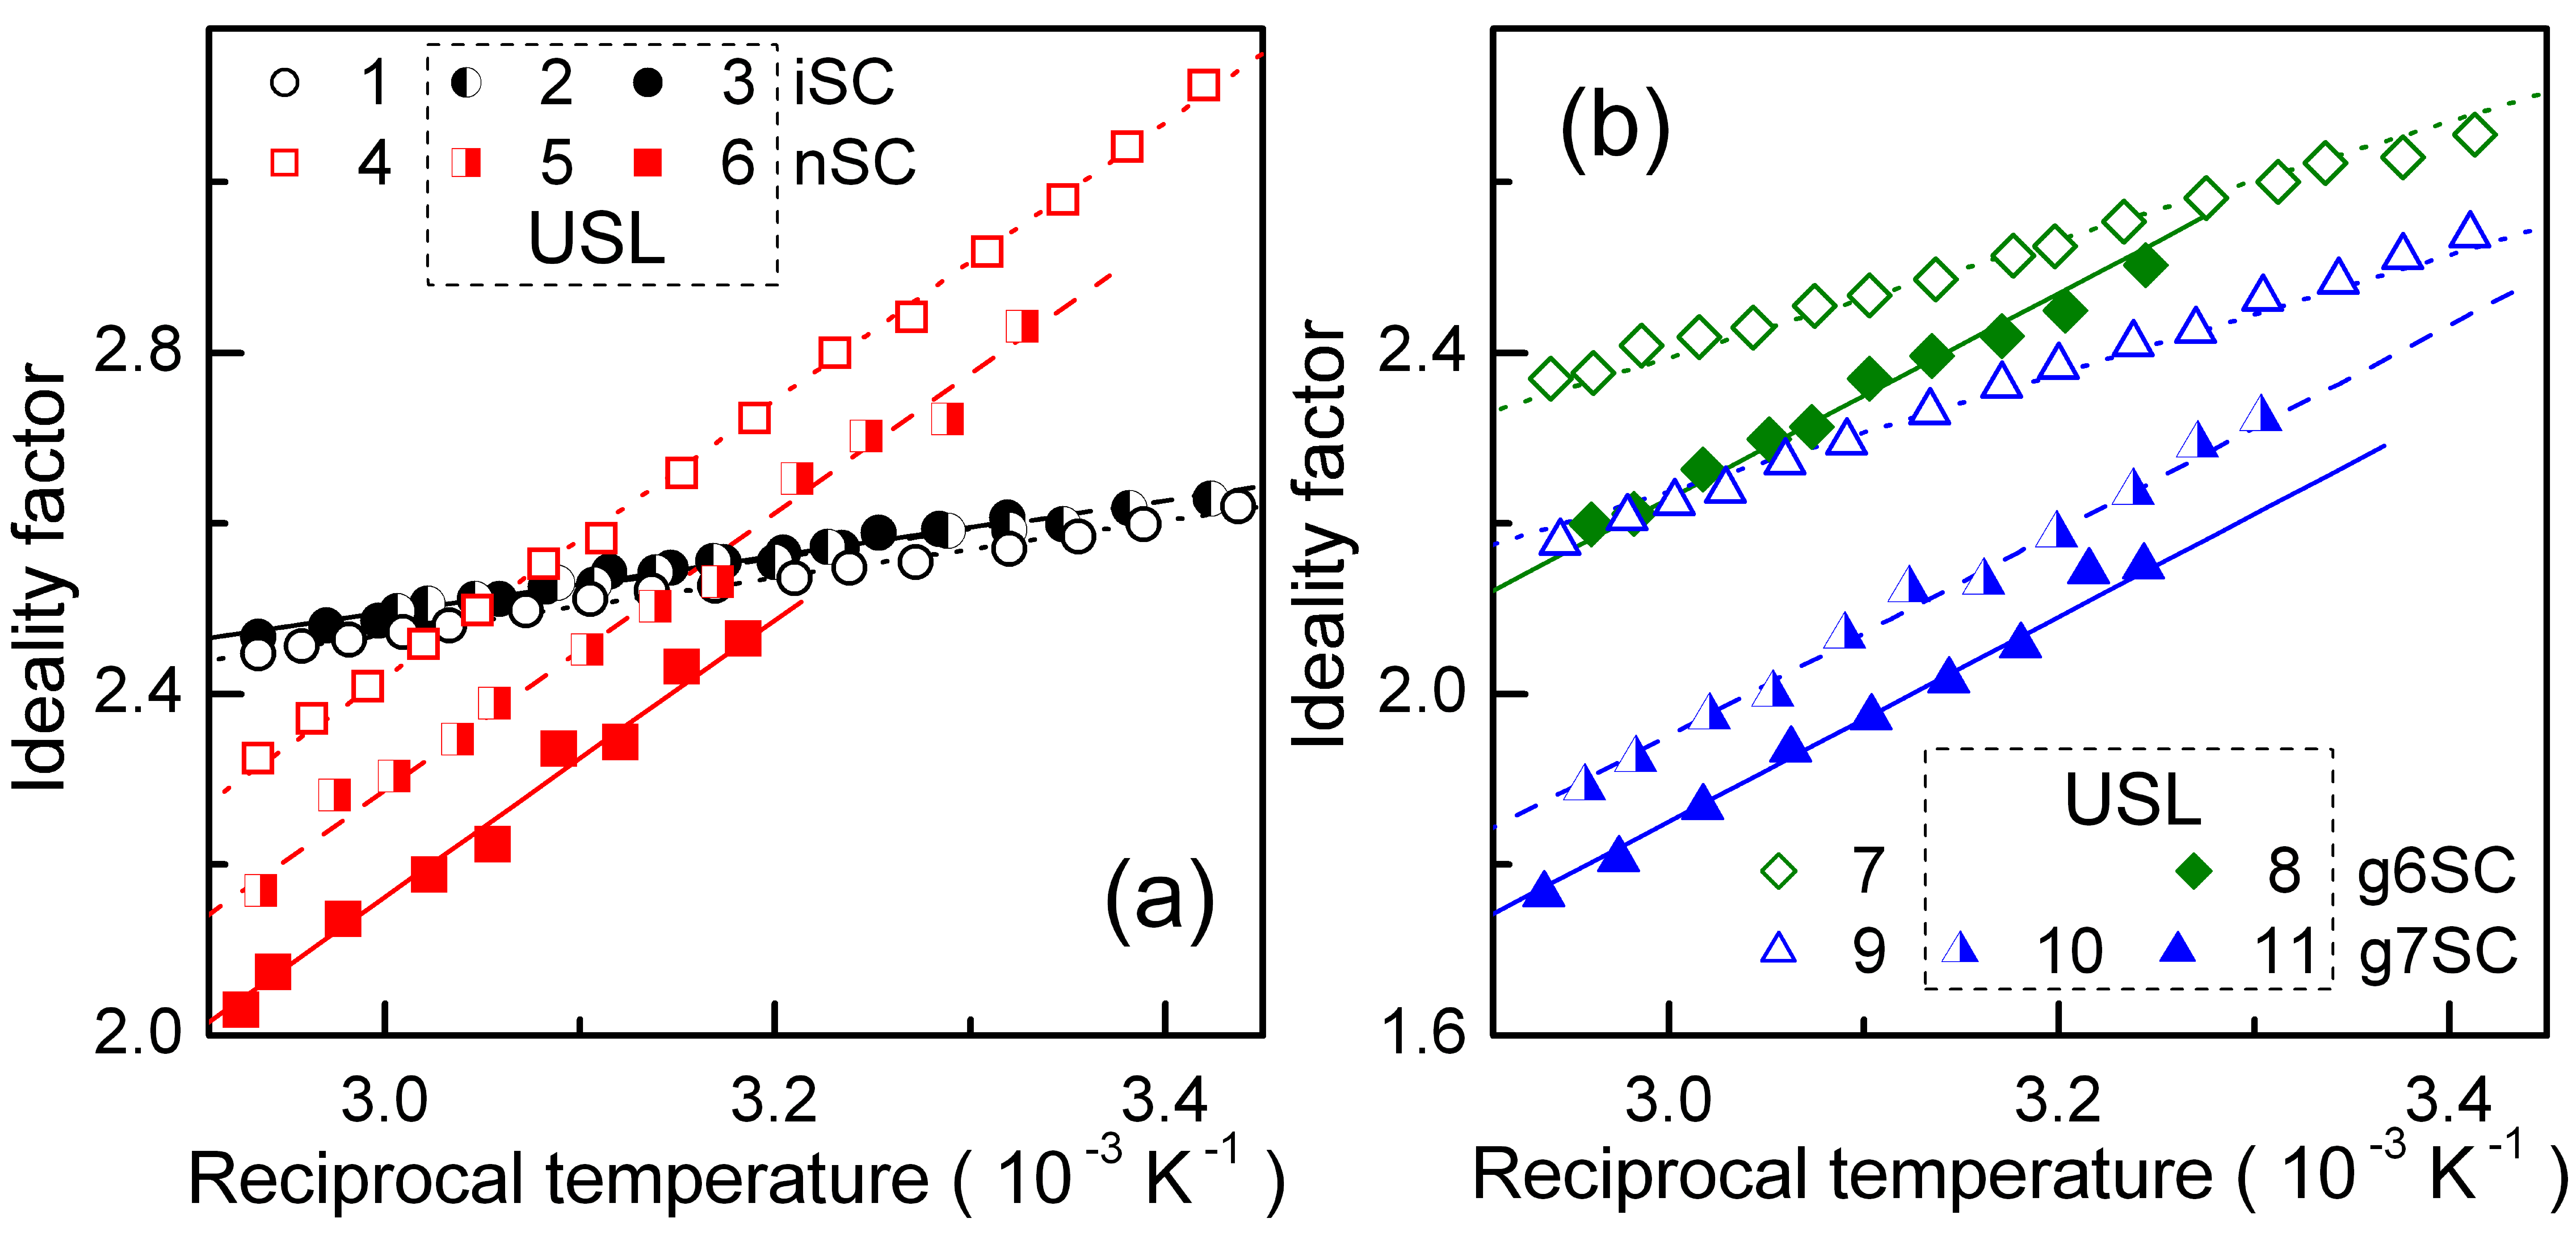
\includegraphics[width=0.7\textwidth]{olikhFig2}%
\caption{\label{fig_n}
Temperature dependences of ideality factor for non--irradiated (curves 1--3, circles),
neutron--irradiated (4--6, squares) and $\gamma$--irradiated (7--11, diamonds and triangles) samples.
The curves 1, 4, 7 and 9 (open marks) are obtained without USL,
curves 2, 3, 5, 6, 8, 10, and 11 correspond to
Ui--1, Ui--2, Un--1, Un--2, Ug6--2, Ug7--1, and Ug7--2 respectively.
The marks are the experimental results, the lines are the fitted curves using Eq.~(\ref{eq_nT}).
}%
\end{figure*}

\begin{figure*}
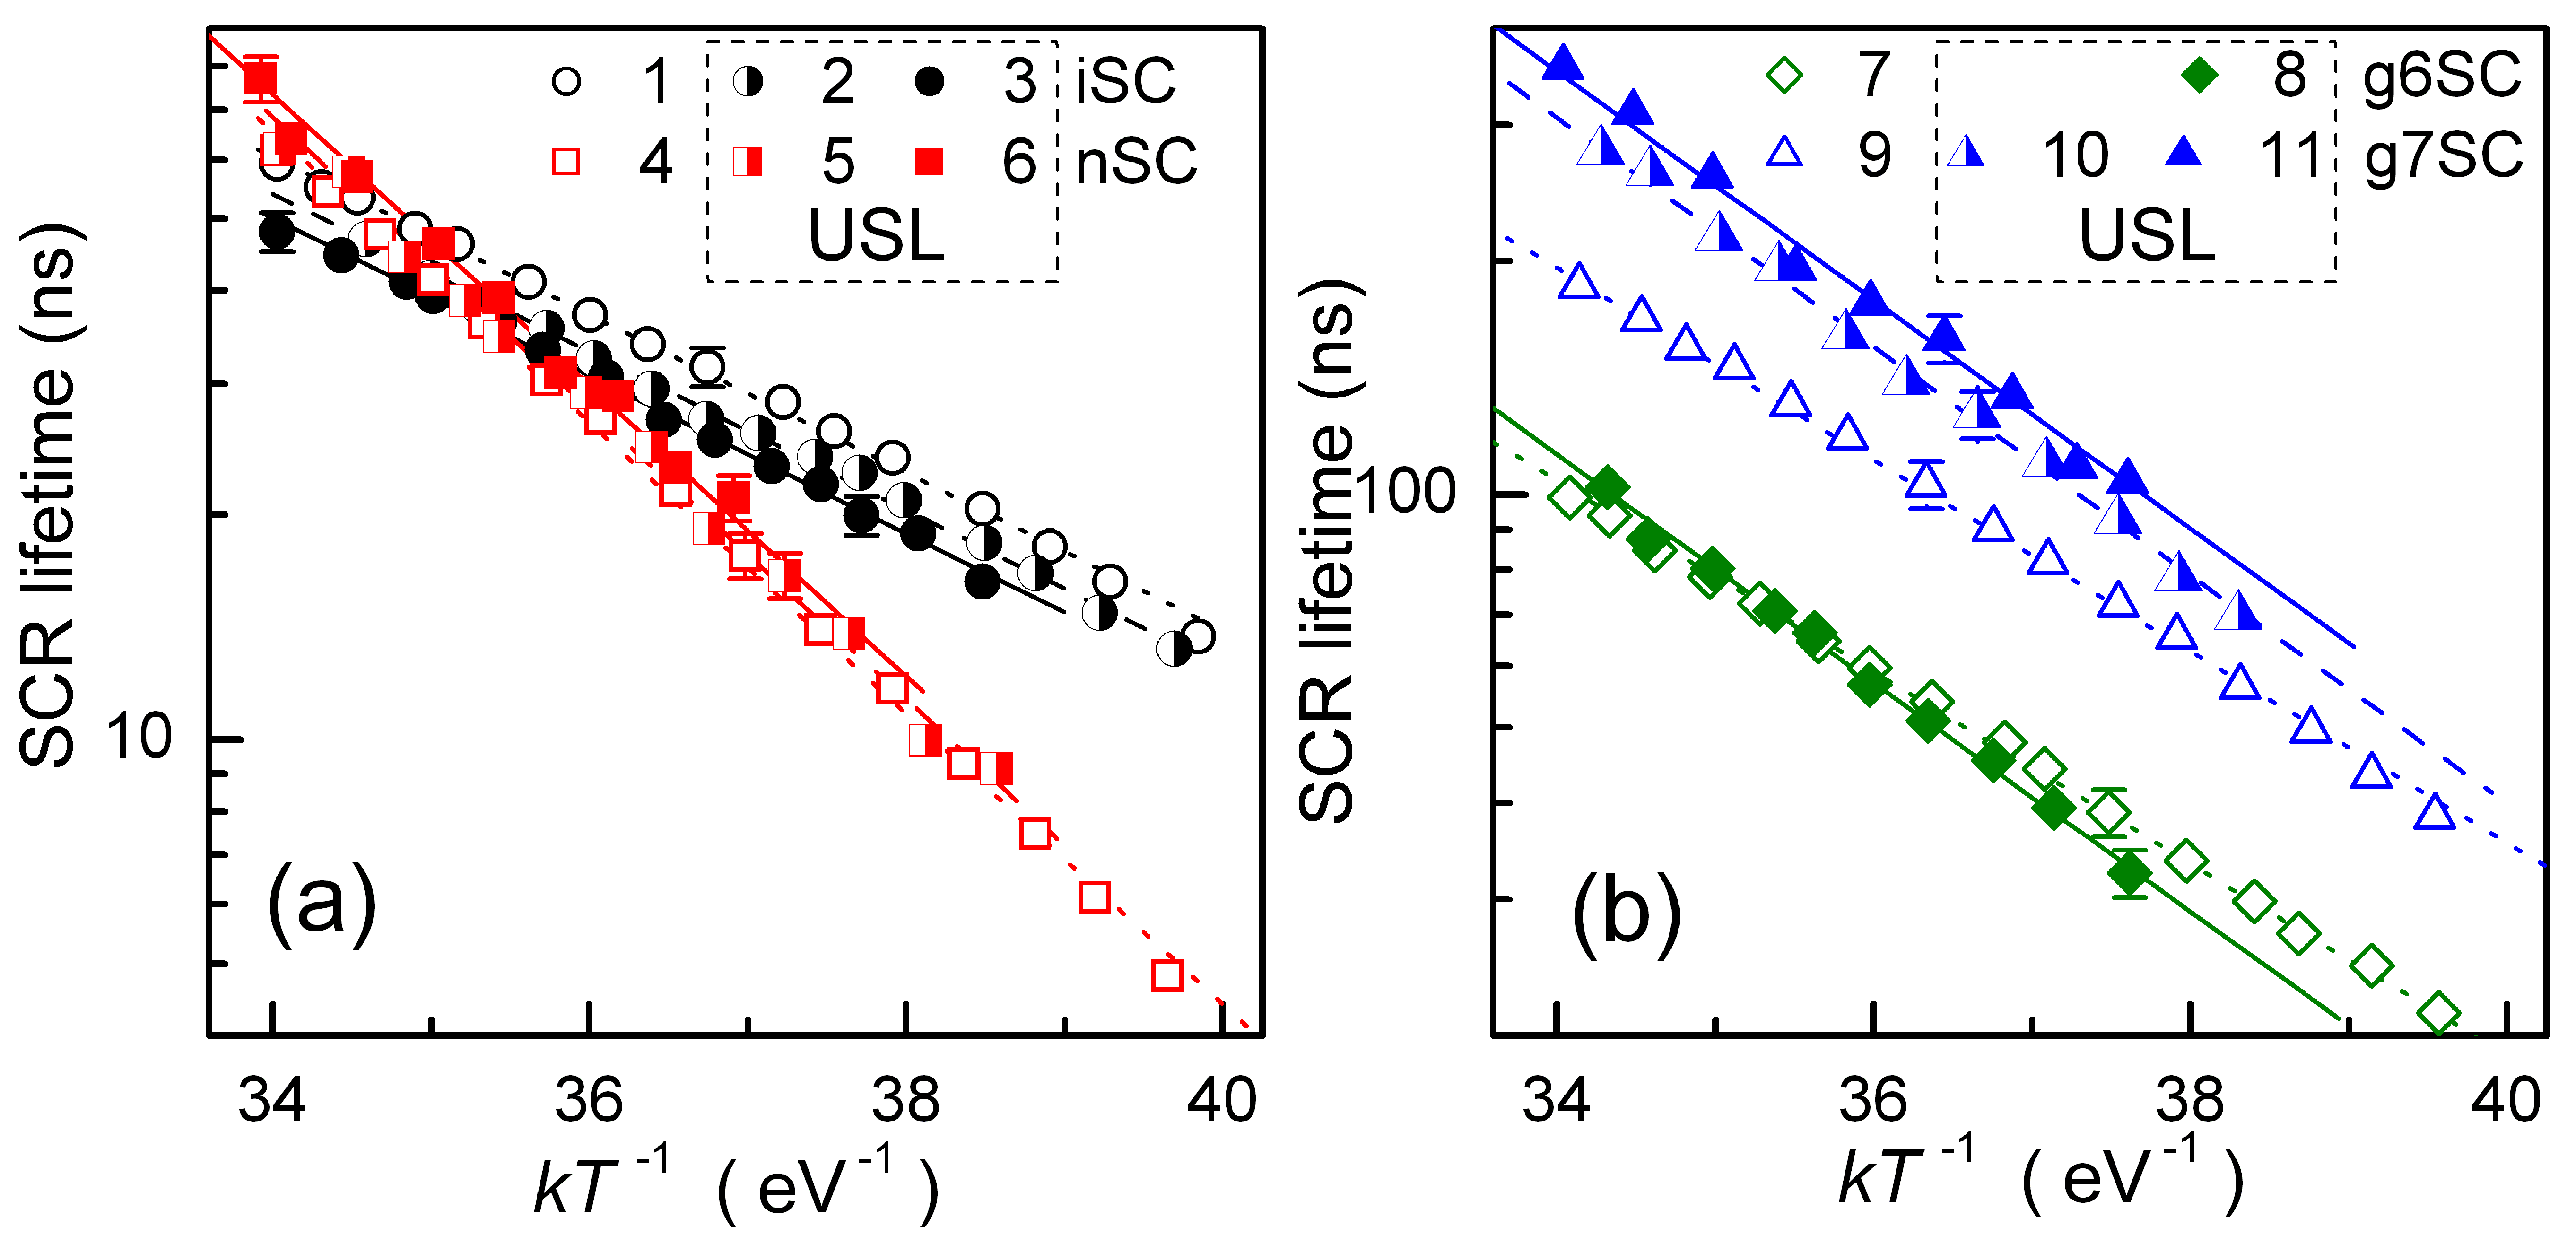
\includegraphics[width=0.7\textwidth]{olikhFig3}%
\caption{\label{fig_TAUg}
Temperature dependences of SCR lifetime for non--irradiated (curves 1--3, circles),
neutron--irradiated (4--6, squares) and $\gamma$--irradiated (7--11, diamonds and triangles) samples.
The curves 1, 4, 7 and 9 (open marks) are obtained without USL,
curves 2, 3, 5, 6, 8, 10, and 11 correspond to
Ui--1, Ui--2, Un--1, Un--2, Ug6--2, Ug7--1, and Ug7--2 respectively.
The marks are the experimental results, the lines are the fitted curves using Eq.~(\ref{eq_TAUgT}).
}%
\end{figure*}

As one can recognize, ideality factor decreases with temperature increase and the plot $n_{\mathrm{id}}$ vs $1/T$  is close to linear.
Thus dependence $n_{\mathrm{id}}(T)$ can be expressed as
\begin{equation}
\label{eq_nT}
    n_{\mathrm{id}}(T)=n_{\mathrm{id},\infty}+T_{\mathrm{id}}/T\:.
\end{equation}
The thermoactivated growth of SCR lifetime is observed over the explored temperature range --- see Fig.~\ref{fig_TAUg}.
The following equation allows to describe sufficiently $\tau_{g}$ temperature dependence:
\begin{equation}
\label{eq_TAUgT}
    \tau_{g}(T)=\tau_{g0}\exp\left(-\frac{E_{\tau g}}{kT}\right)\:.
\end{equation}
The $T_{\mathrm{id}}$ and $E_{\tau g}$ values, which have been determined for both non-irradiated and irradiated samples with as well as without USL are listed in Table~\ref{tabTpar}.

\begin{table*}
\caption{\label{tabTpar}Characteristics of temperature dependences of $n^+$--$p$--Si structure parameters.
}
\begin{ruledtabular}
\begin{tabular}{cccccc}
Sample&USL&$T_{\mathrm{id}}$ (K)&$E_{\tau g}$ (eV)&$R_{293,\mathtt{Al}}$ (k$\Omega$)&$\sigma_{\mathtt{dis}}$ ($10^4$~K/$\Omega$)\\
%Sample&USL&$T_{\mathrm{id}}$&$E_{\tau g}$&$R_{293,\mathtt{Al}}$&$\sigma_{\mathtt{dis}}$\\
%&&(K)& (eV)&(k$\Omega$)&($10^4\Omega^{-1}$m$^{-1}$)\\
\hline
%\multirow{3}{*}{iSC}&non&$330\pm30$&$0.24\pm0.01$\\
iSC&non&$330\pm30$&$0.24\pm0.01$&$27\pm3$&$41\pm4$\\
&Ui--1&$310\pm30$&$0.24\pm0.01$&$27\pm3$&$50\pm4$\\
&Ui--2&$360\pm30$&$0.24\pm0.01$&$26\pm3$&$58\pm4$\\
%\multirow{3}{*}{nSC}&non&$1610\pm70$&$0.45\pm0.02$\\
nSC&non&$1610\pm70$&$0.45\pm0.02$&$2.2\pm0.4$&$65\pm7$\\
&Un--1&$1600\pm70$&$0.44\pm0.02$&$2.3\pm0.4$&$95\pm10$\\
&Un--2&$1680\pm70$&$0.44\pm0.02$&$2.2\pm0.4$&$130\pm10$\\
%\multirow{2}{*}{g6SC}&non&$610\pm40$&$0.28\pm0.01$\\
g6SC&non&$610\pm40$&$0.28\pm0.01$&$0.7\pm0.1$&$19\pm2$\\
&Ug6--2&$1080\pm50$&$0.33\pm0.02$&$0.8\pm0.1$&$24\pm2$\\
%\multirow{3}{*}{g7SC}&non&$770\pm50$&$0.29\pm0.01$\\
g7SC&non&$770\pm50$&$0.29\pm0.01$&$0.41\pm0.06$&$26\pm3$\\
&Ug7--1&$1260\pm60$&$0.34\pm0.02$&$0.39\pm0.06$&$45\pm4$\\
&Ug7--2&$1270\pm60$&$0.35\pm0.02$&$0.38\pm0.06$&$55\pm4$\\
\end{tabular}
\end{ruledtabular}
\end{table*}

We want to stress, that

\noindent
(i)~irradiation leads to $T_{\mathrm{id}}$ and $E_{\tau g}$ changes, the g6SC's ideality factor characteristic temperature and SCR lifetime characteristic energy values are closely related to g7SC ones at similar conditions;

\noindent
(ii)~USL affects $n_{\mathrm{id}}$ and $\tau_g$ values, absolute AI changes of ideality factor $\Delta n_{\mathrm{id}}=n_{\mathrm{id},\mathtt{US}}-n_{\mathrm{id},in}$ and
relative AI changes of SCR lifetime $\varepsilon_{\tau g}=(\tau_{g,\mathtt{US}}-\tau_{g,in})/\tau_{g,in}$
(where subscripts ``$\mathtt{US}$'' and ``$in$'' identify with values,
%$n_{\mathtt{US}}(T)$ and $n_{in}(T)$ are the ideality factor,
which are obtained at the same temperature with and without USL respectively)
are listed in Table~\ref{tabAIchange};

\noindent
(iii)~$\Delta n_{\mathrm{id}}$ and $\varepsilon_{\tau g}$ vary with $W_{\mathtt{US}}$ enhancement, whereas $T_{\mathrm{id}}$ and $E_{\tau g}$ values do not depend on US intensity practically.


\noindent
(iv)~USL results in both $T_{\mathrm{id}}$ and $E_{\tau g}$ increase in $\gamma$--irradiated samples --- see Fig.~\ref{fig_n}(b) and Fig.~\ref{fig_TAUg}(b), but same effect is not observed in non--irradiated and neutron--irradiated samples --- see Fig.~\ref{fig_n}(a) and Fig.~\ref{fig_TAUg}(a);

\noindent
(v)~$\Delta n_{\mathrm{id}}$ and $\varepsilon_{\tau g}$ have an opposite sign for non--irradiated and irradiated samples
(for SCg6 not in whole temperature range);

\noindent
(vi)~ideality factor is varied by USL more effectively in irradiated samples;


%\noindent
%(vii)~US influence efficiency for $\gamma$--irradiated samples rises with dose;




\begin{table}
\caption{\label{tabAIchange}Acoustically induced change of $n^+$-$p$--Si structure parameters (at 330~K).
}
\begin{ruledtabular}
\begin{tabular}{cccccc}
Sample&USL&$\Delta n_{\mathrm{id}}$ &$\varepsilon_{\tau g}$ &$\varepsilon_{\tau n}$ &$\varepsilon_{\sigma\mathtt{dis}}$ \\
&&\mbox{($\pm0.01$)}&($\pm5$\%)&($\pm0.2$)&($\pm10$\%)\\
\hline
%\multirow{2}{*}{iSC}&Ui--1&0.02&-14&-43&-15\\
iSC&Ui--1&0.02&-14&0.7&20\\
&Ui--2&0.03&-17&1.4&40\\
%\multirow{2}{*}{nSC}&Un--1&-0.13&5&-60&-19\\
nSC&Un--1&-0.13&5&1.5&50\\
&Un--2&-0.26&13&3.0&100\\
g6SC&Ug6--2&-0.15&2&2.3&30\\
%\multirow{2}{*}{g7SC}&Ug7--1&-0.26&49&0.9&-5\\
g7SC&Ug7--1&-0.26&49&0.9&70\\
&Ug7--2&-0.36&70&1.9&110\\
\end{tabular}
\end{ruledtabular}
\end{table}


For purpose of the present consideration, it is important to discuss the recombination mechanism in the SCR of the investigated samples.
According to classical SRH theory, an ideality factor must be less than 2 and
$\tau_g$ temperature dependence is expected \cite{TAUg:Schroder,TAUg:Aharoni} to be described by the relation  $\tau_g\simeq2\,\tau_n\sqrt{\sigma_n/\sigma_p}\cosh\left[\left(E_t-E_i\right)/kT\right]$
(where $\sigma_n$, $\sigma_p$, and  $E_t$ are the electron and hole capture cross sections (CCSs) and the energy  level of  the  recombination  center,
$E_i$  is the  intrinsic  energy level).
In the our case, $n_{\mathrm{id}}$ is lager than 2 and $\tau_g$ increases with temperature.
Therefore SRH theory is inapplicable to the investigated samples.
Several attempts to explain large $n_{\mathrm{id}}$ have been made with various models.\cite{Heide,Beier,Shah,Kaminski_n}
But all observed features of SCR recombination (ideality factor large value, independence on light intensity, dependence on temperature
as well as carrier lifetime small value) can be explained by the model of coupled defect level recombination (CDLR) \cite{CDLR:JAP1995,CDLR:JAP} only.
This model provides a rapid  direct  charge  transfer  between  defect levels.
Such phenomenon has been observed experimentally firstly \cite{DAPR:Chen1991,DAPR:Chen1994} and then it was recruited to explain process in semiconductor diodes. \cite{CDLR:JAP1995,CDLR:JAP,CDLR:SSP}

According to the CDLR model, recombination is the result of carrier exchange between two defect level and crystal bands.
In particular, it is proposed \cite{CDLR:JAP} that the recombination rate is dominated by sites where an acceptor--like defect is coupled to a donor-like defect.
In the simplified case of
no carrier exchange between the donor level $E_t^{\mathtt{D}}$ and the valence band
as well as between the acceptor level $E_t^{\mathtt{A}}$ and the conduction band,
%In the simplified case, when
%carrier exchanges between the donor level and the conduction band,
%between the acceptor level and the valence band,
%and between the donor level and the acceptor level are allowed only,
the recombination rate $R$ can be expressed\cite{CDLR:JAP1995} as
\begin{eqnarray}
R&=&\frac{R_{12}-\sqrt{R_{12}^{\,2}-4\tau_{n}^{\mathtt{D}}\tau_{p}^{\mathtt{A}}(np-n_i^2)(1-\epsilon)}}{2\tau_{n}^{\mathtt{D}}\tau_{p}^{\mathtt{A}}(1-\epsilon)}\;,\label{eqR}\\
R_{12}&=&\frac{(n+n_{\mathtt{D}})(p+p_{\mathtt{A}})}{R_{\mathtt{DA}}}+
\tau_{n}^{\mathtt{D}}(p+p_{\mathtt{D}})+\tau_{p}^{\mathtt{A}}(n+n_{\mathtt{A}}),\label{eqR12}\\
\tau_{n}^{\mathtt{D}}&=&(N_{\mathtt{D}}\,\sigma_{n}^{\mathtt{D}}\,\upsilon_{\mathrm{th},n})^{-1},\,\,\,\,
\tau_{p}^{\mathtt{A}}=(N_{\mathtt{A}}\,\sigma_{p}^{\mathtt{A}}\,\upsilon_{\mathrm{th},p})^{-1},\label{eqTAU}
%\\
%n_{\mathtt{D,A}}&=&N_c(g_0^{\mathtt{D,A}}/g_1^{\mathtt{D,A}})\cdot\exp[-E_t^{\mathtt{D,A}}/kT],\label{eq_nDA}\\
%p_{\,\mathtt{D,A}}&=&N_v(g_1^{\mathtt{D,A}}/g_0^{\mathtt{D,A}})\cdot\exp[-(E_g-E_t^{\mathtt{D,A}})/kT],\label{eq_pDA}\\
%\epsilon&=&(g_1^{\mathtt{D}}\,g_0^{\mathtt{A}})/(g_0^{\mathtt{D}}\,g_1^{\mathtt{A}})\cdot\exp[-(E_t^{\mathtt{A}}-E_t^{\mathtt{D}})/kT]\,,\label{eqEPS}
\end{eqnarray}
where
$R_{\mathtt{DA}}$ is the coupling parameter,
%$n_{\mathtt{D,A}}=N_c\frac{g_0^{\mathtt{D,A}}}{g_1^{\mathtt{D,A}}}\exp\left(\frac{E_c-E_t^{\mathtt{D,A}}}{kT}\right)$
%$\tau_{n,p}^{\mathtt{D,A}}=(N_{\mathtt{DAP}}\sigma_{n,p}^{\mathtt{D,A}}\upsilon_{th,n,p})^{-1}$ ,
%$N_{\mathtt{DAP}}=(N_{\mathtt{D}}+N_{\mathtt{A}})/2$ is the donor--acceptor--pair (DAP) density,
$N_{\mathtt{D}}$ and $N_{\mathtt{A}}$ are the density of the donor and acceptor--like defects,
$\sigma_{n}^{\mathtt{D}}$ and $\sigma_{p}^{\mathtt{A}}$ are electron CCS of donor and hole CCS of acceptor,
$\upsilon_{\mathrm{th},n}$ and $\upsilon_{\mathrm{th},p}$ are the thermal electron and hole velocity,
$n_{\mathtt{D,A}}$, $p_{\,\mathtt{D,A}}$, and $\epsilon$ depend on $E_t^{\mathtt{D}}$, $E_t^{\mathtt{A}}$, and level degeneracy  factors.
%$\epsilon=\frac{g_1^{\mathtt{D}}g_0^{\mathtt{A}}}{g_0^{\mathtt{D}}g_1^{\mathtt{A}}}\exp\left(\frac{E_t^{\mathtt{D}}-E_t^{\mathtt{A}}}{kT}\right)$,
%$E_t^{\mathtt{D}}$ and $E_t^{\mathtt{A}}$ are the donor and acceptor levels  measured  from  the  conduction  band edge,
%$g_{0,1}$ are degeneracy  factors  of  the empty  and occupied  levels.
As $\tau_g\propto R^{-1}$, last ones are expected to provide a thermoactivated SCR lifetime behavior.
Unfortunately, the functional relation between $I$--$V$ characteristic parameters and attributes of defects, which take part in CDLR, is not suggested.

According to Steingrube \emph{et al}.\cite{CDLR:JAP},
SSC for defect in a pair differs from that for isolated defect and depends on the distance between donor and acceptor $r$:
\begin{equation}
\label{eqSigma}
\sigma_{n,p}^{\mathtt{D,A}}(r)=C_{n,p}^{\mathtt{D,A}}\,r^2\,,
\end{equation}
where $C_{n}^{\mathtt{D}}$ and $C_{p}^{\mathtt{A}}$ are some constant.
Besides, $R_{\mathtt{DA}}$ is proportional to the overlap integral of the wave functions.
If both defects are characterized by H--like radial--symmetric wave function and equal Bohr radius $a_0$,
the following expression can be used: \cite{CDLR:JAP}
\begin{equation}
\label{eqRda}
R_{\mathtt{DA}} (r) \propto N_{\mathtt{D}}N_{\mathtt{A}}\left[1+\frac{r}{a_0}+\frac{1}{3}\left(\frac{r}{a_0}\right)^2\right]
   e^{-r/a_0}\,.
%   \exp\left(-\frac{r}{a_0}\right)\,.
\end{equation}


%According to Steingrube \emph{et al}.\cite{CDLR:JAP},
%$\sigma_{n}^{\mathtt{D}}$, $\sigma_{p}^{\mathtt{A}}$,  and $R_{\mathtt{DA}}$
%depend on the distance between donor and acceptor $r$.
%If wave functions for both defects are characterized by H--like radial--symmetric and equal Bohr radius $a_0$,
%%In the case of H--like radial--symmetric wave functions for the defects with equal Bohr radii $a_0$,
%the following expression can be used \cite{CDLR:JAP}:
%\begin{eqnarray}
%\sigma_{n,p}^{\mathtt{D,A}}&=& \sigma_{n,p}^{0\mathtt{D,A}}\left(\frac{r}{r_0^{\mathtt{D,A}}}\right)^2\,,\label{eqSigma}\\
%R_{\mathtt{DA}} &=& C_{\mathtt{DA}}N_{\mathtt{D}}N_{\mathtt{A}}\left[1+\frac{r}{a_0}+\frac{1}{3}\left(\frac{r}{a_0}\right)^2\right]
%   \exp\left(-\frac{r}{a_0}\right)\,,\label{eqRda}
%\end{eqnarray}
%where
%$\sigma_{n}^{0\mathtt{D}}$ and $\sigma_{p}^{0\mathtt{A}}$ are CCS of the isolated (non--coupled) donor and acceptor,
%$r_0^{\mathtt{D}}$, $r_0^{\mathtt{A}}$,  and $C_{\mathtt{DA}}$ are some constant.

In our opinion, the observed reversible AI $n_{\mathrm{id}}$ and $\tau_g$ modifications are induced by
donor--acceptor distance alteration in samples under USL.
Really, according to data,\cite{MirzadeJAP2011,PeleshchakUJF2016} the force acting on the point defect during USL can be expressed as
\begin{equation}
\label{eqFd}
F_d=\chi\,\Delta\Omega_d\frac{\partial \xi(z,t)}{\partial z}\,,
\end{equation}
where
$\chi$ is the bulk elasticity modulus,
$\Delta\Omega_d$ is the crystal volume change per defect,
$\xi$ is the crystal lattice deformation,
and AW propagates along $z$ direction.
$\partial \xi(z,t)/\partial z\propto \xi_{\mathtt{US}}$.
For interstitial atoms and substitutional impurities with the ionic radius exceeding the ionic radius of matrix
atoms, the $\Delta\Omega_d > 0$, whereas,
for vacancies and substitutional impurities with ionic radius smaller than the ionic radius of matrix atoms,
$\Delta\Omega_d < 0$.
Therefore, a point defect vibrates under USL condition and oscillation amplitude and phase are determined by both defect character and AW intensity.

\begin{figure}
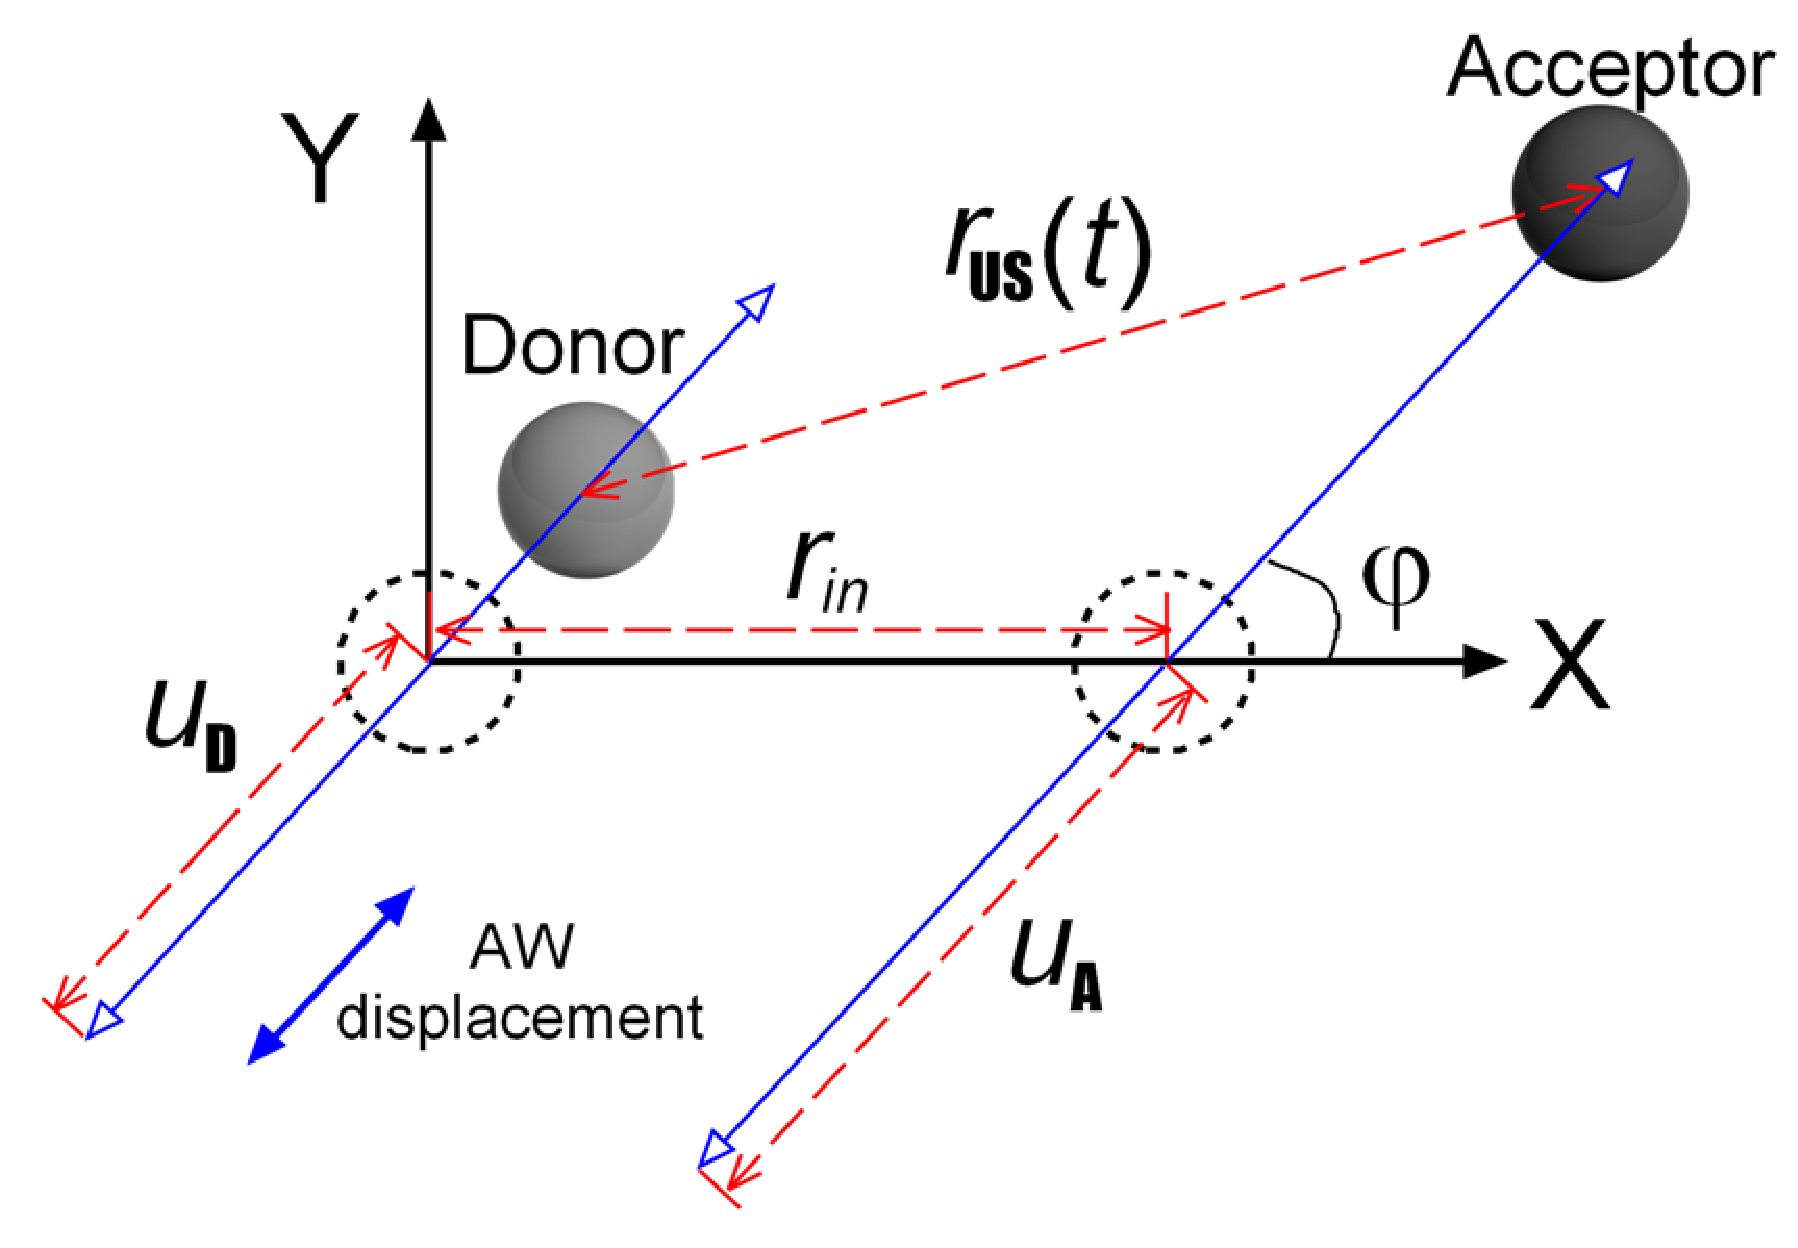
\includegraphics[width=0.45\textwidth]{olikhFig4}%
\caption{\label{fig_Model}
Model of CDLR center behavior under US action.
}%
\end{figure}

Some qualitative conclusion can be drawn from the simplest model, which is shown in Fig.~\ref{fig_Model}.
Initially donor and acceptor are situated at distance $r_{in}$.
Axis X is drawn through point defect inial positions.
During USL defects would vibrate with amplitudes $u_\mathtt{D}$ and $u_\mathtt{A}$.
Vibration axis coincides with AW displacement direction and forms angle $\varphi$ with  X--axis.
The amplitudes depend on $\xi_{U\!S}$, defect elastic strain ($\Delta\Omega_d^\mathtt{D}$ and $\Delta\Omega_d^\mathtt{A}$), defect coupling  and can be different.
According to suggested model, the donor--acceptor distance in the sample with USL $r_\mathtt{US}$ depends on time $t$:
%\begin{eqnarray}
%\label{eqrUS}
%r_\mathtt{US}(t)&=&\left\{[r_{in}+u_\mathtt{A}\cos(\omega_\mathtt{US}t+\delta)-u_\mathtt{D}\cos(\omega_\mathtt{US}t)]^2\cos^2\varphi \right.\nonumber\\
%   && \left.+ [u_\mathtt{A}\cos(\omega_\mathtt{US}t+\delta)-u_\mathtt{D}\cos(\omega_\mathtt{US}t)]^2\sin^2\varphi\right\}^{0.5}\,,
%\end{eqnarray}
\begin{multline}
\label{eqrUS}
r_\mathtt{US}(t)=\left\{[r_{in}+u_\mathtt{A}\cos(\omega_\mathtt{US}t+\delta)-u_\mathtt{D}\cos(\omega_\mathtt{US}t)]^2\cos^2\varphi \right.\\
    \left.+ [u_\mathtt{A}\cos(\omega_\mathtt{US}t+\delta)-u_\mathtt{D}\cos(\omega_\mathtt{US}t)]^2\sin^2\varphi\right\}^{0.5}\,,
\end{multline}
where $\omega_\mathtt{US}$ is the US cyclic frequency,
$\delta$ is the phase shift between donor and acceptor vibration.

We use Eqs.~(\ref{eqSigma})--(\ref{eqRda}) to estimate AI relative changes of CCS
$\varepsilon_\sigma=[\sigma_{\mathtt{US}}-\sigma(r_{in})]/\sigma(r_{in})$
and coupling parameters $\varepsilon_{\mathtt{RDA}}=[R_{\mathtt{DA,US}}-R_\mathtt{DA}(r_{in})]/R_\mathtt{DA}(r_{in})$,
where $\sigma_{\mathtt{US}}$ and $R_{\mathtt{DA,US}}$ are averaged over the AW period $T_\mathtt{US}$:
\begin{equation*}
\label{eqAver}
\sigma_{\mathtt{US}}=\frac{1}{T_\mathtt{US}}\int^{T_\mathtt{US}}_0\!\!\!\!\!\!\sigma(r_\mathtt{US}(t))dt\,,
R_{\mathtt{DA,US}}=\frac{1}{T_\mathtt{US}}\int^{T_\mathtt{US}}_0\!\!\!\!\!\!R_{\mathtt{DA}}(r_\mathtt{US}(t))dt\,.
\end{equation*}
While estimating, relaxation time in the CDLR sub--system is assumed to be considerably less than $T_\mathtt{US}$
and the previously used\cite{CDLR:JAP} value $a_0=3.23$~nm is utilized.
Besides, the chosen $u_\mathtt{D}$ and $u_\mathtt{A}$ values are commensurate with $u_\mathtt{US}$.
But it is taken into account, that a displacement of the point defect without covalent bond could exceed a matrix atom displacement.
At last, no US  absorption by defect is assumed.
In this simple case $\delta$ equals to $0^\circ$, if $(\Delta\Omega_d^\mathtt{D}\cdot\Delta\Omega_d^\mathtt{A})>0$,
or to $180^\circ$, if $(\Delta\Omega_d^\mathtt{D}\cdot\Delta\Omega_d^\mathtt{A})<0$.
In addition, $\varepsilon_{\mathtt{RDA}}$ dependence on
%oscillation amplitudes
$u_\mathtt{D}$ and $u_\mathtt{A}$
is only determined by $|u_\mathtt{D}-u_\mathtt{A}|$ ($\delta=0^\circ$ case) or $|u_\mathtt{D}+u_\mathtt{A}|$ ($\delta=180^\circ$ case).
Moreover, these dependences are identical in both cases.
The typical simulation results are shown in  Fig.~\ref{fig_Erda}.

%In addition, both $\varepsilon_{\mathtt{RDA}}$ and $\varepsilon_{\sigma}$ dependences on oscillation amplitudes
%are only determined by $|u_\mathtt{D}+u_\mathtt{A}|$ (if $\delta=180^\circ$) or $|u_\mathtt{D}-u_\mathtt{A}|$ (if $\delta=0^\circ$).
%Moreover, these dependences are identical in both cases.

\begin{figure}
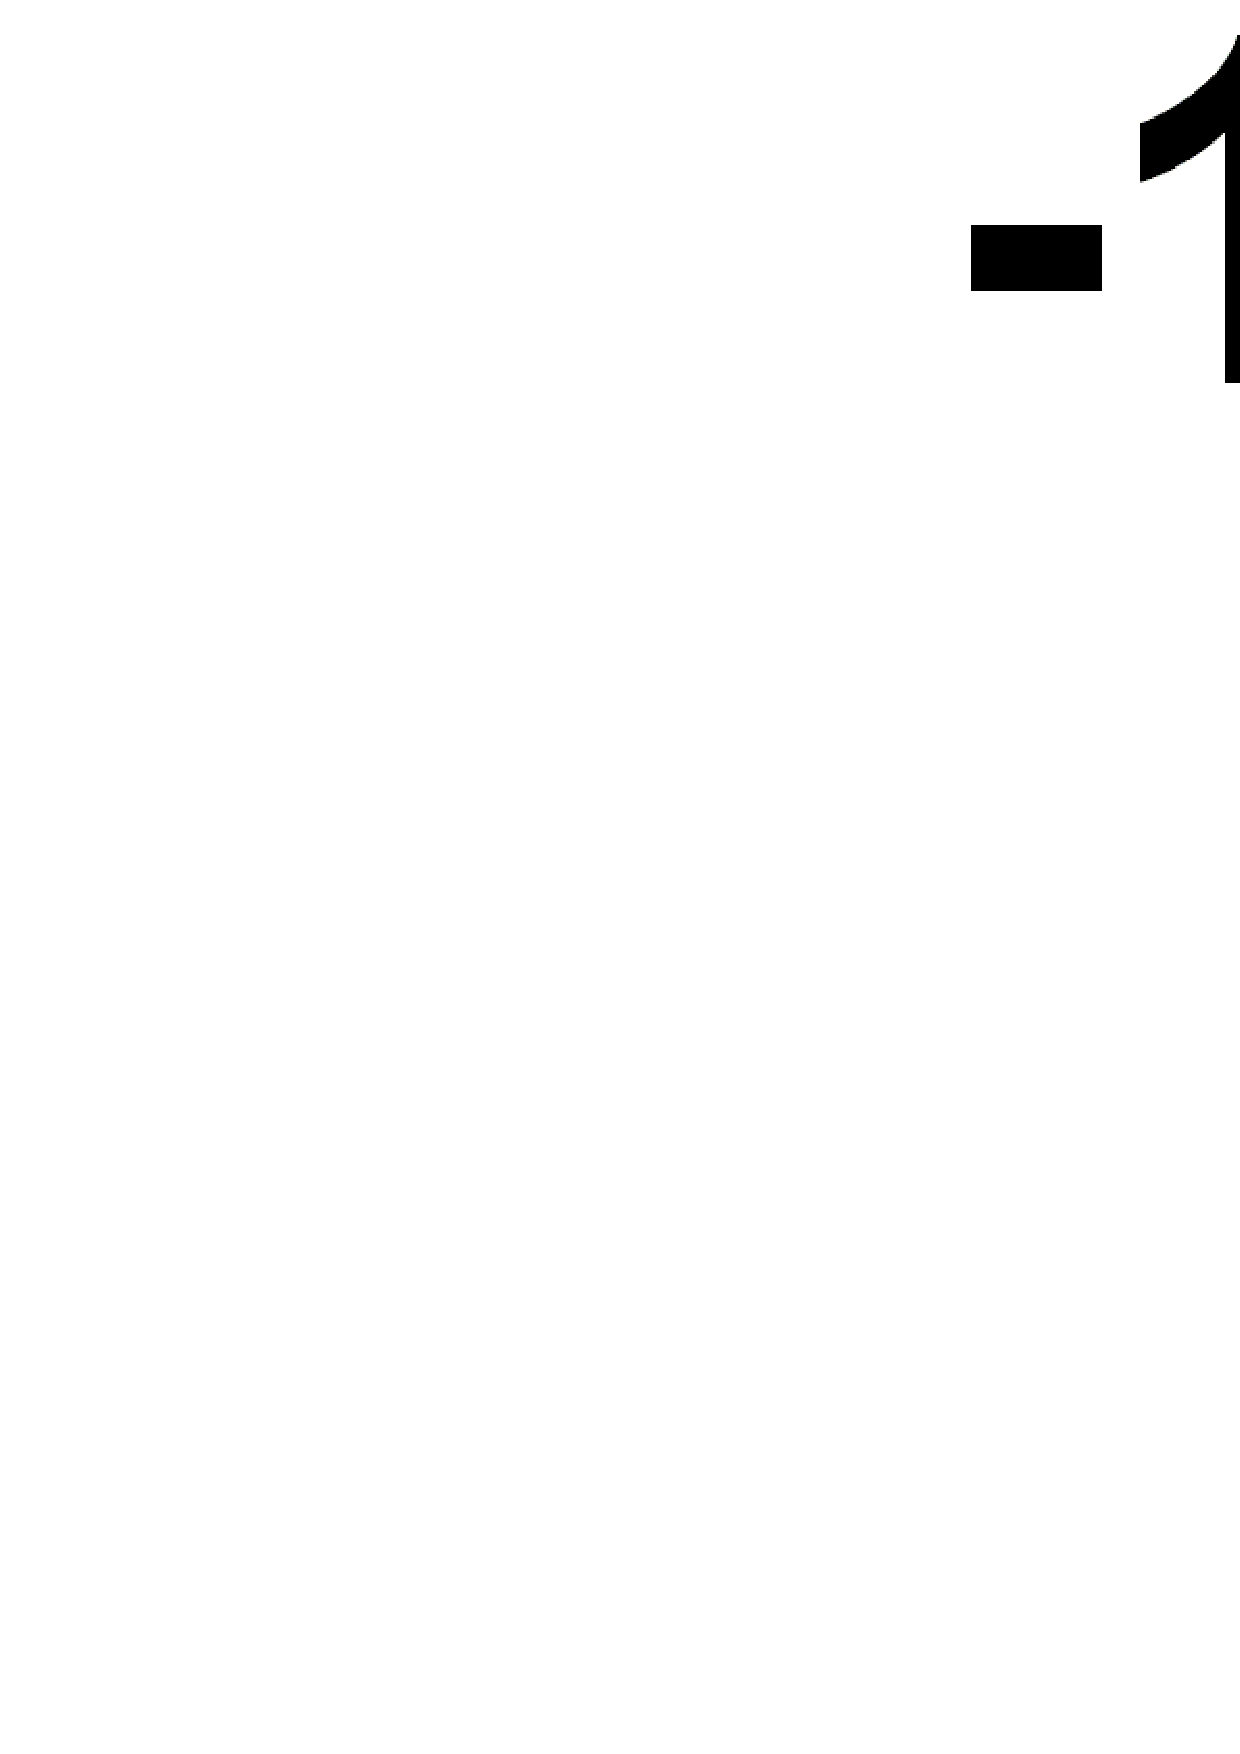
\includegraphics[width=0.45\textwidth]{olikhFig5}%
\caption{\label{fig_Erda}
Simulated dependencies of AI changes of coupling parameter on the vibration amplitudes.
Axis $|u_\mathtt{D}+u_\mathtt{A}|$ corresponds to $\delta=0^\circ$ case, whereas axis $|u_\mathtt{D}+u_\mathtt{A}|$ corresponds to $\delta=180^\circ$ case.
The parameters are set to $a_0=3.23$~nm,
$r_{in}=5$~nm (open marks), $15$~nm (semi--filled marks), and $25$~nm (filled marks),
$\varphi=0^\circ$ (circles), $90^\circ$ (squares).
Triangles correspond to mean $\varepsilon_{\mathtt{RDA}}$ value for $[0^\circ\div 180^\circ]$ $\varphi$ range.
}%
\end{figure}

$\varepsilon_{\sigma}$ depends on oscillation amplitudes with a similar features and
does not depend on $\varphi$:
\begin{equation}
\label{eqEpsSig}
\varepsilon_{\sigma}=(u_\mathtt{D}\pm u_\mathtt{A})^2/2\,r_{in}^2=K_\mathtt{US}^\mathtt{DA}W_{\mathtt{US}}\,,
\end{equation}
where``$+$'' and ``$-$'' correspond to $\delta=180^\circ$ and $\delta=0^\circ$ respectively,
$K_\mathtt{US}^\mathtt{DA}$ characterizes defect couple--ultrasound interaction and depends on properties defects as well as crystal matrix.
It is taken into account in Eq.~(\ref{eqEpsSig}), that $u_\mathtt{D},u_\mathtt{A}\propto \xi_\mathtt{US}\propto\sqrt{W_\mathtt{US}}$.

Before analysing, it is worth keeping in mind, that
CLDR current flows locally in the locations of extended defects.\cite{CDLR:JAP,CDLR:SSP}
On the other hand, dislocations are often situated in the SCR region perpendicularly to $p-n$ junction plane
and investigated samples are not exception (see Section~\ref{Rsh}).
If CDLR in the dislocation locations is assumed, then dislocations with edge component would influence on pair spatial orientation.
Thus axis of donor--acceptor pair with $(\Delta\Omega_d^\mathtt{D}\cdot\Delta\Omega_d^\mathtt{A}>0)$  should be predominantly situated parallel to a dislocation line,
whereas pair of coupled defects with $(\Delta\Omega_d^\mathtt{D}\cdot\Delta\Omega_d^\mathtt{A}<0)$ should be normal.
As AW displacement is parallel to the $p-n$ junction plane,
the most excited curiosity variants are following:


%To limit concerned variant, the simple geometry would be under consideration.
%According to \cite{CDLR:JAP,CDLR:SSP}, CLDR current flows locally in the locations of extended defects,
%where a poind defect concentration is increased essentially and donor and acceptor defects can to couple to each other.
%On the other hand, dislocations are often situated in the SCR region perpendicularly to $p-n$ junction plane --- see Section~\ref{Rsh} for details.
%If CDLR in the locations of dislocation is assumed then dislocations with edge component influence on pair spatial orientation.
%Thus axes of donor--acceptor pair with $\Delta\Omega_d^\mathtt{D}\cdot\Delta\Omega_d^\mathtt{A}>0$  should be predominantly situated parallel to a dislocation line,
%whereas one of coupled defects with $\Delta\Omega_d^\mathtt{D}\cdot\Delta\Omega_d^\mathtt{A}>0$ should be normal.
%Keeping in mind, that AW displacement is parallel to the $p-n$ junction plane,
%the most excited curiosity variants are following:

\noindent  $\delta=0^\circ$, $\varphi=90^\circ$ ($\Delta\Omega_d^\mathtt{D}\cdot\Delta\Omega_d^\mathtt{A}>0$ case);

\noindent  $\delta=180^\circ$, $\varphi\in[0^\circ\div 180^\circ]$ ($\Delta\Omega_d^\mathtt{D}\cdot\Delta\Omega_d^\mathtt{A}<0$ case).

\noindent
In other words, all curves in Fig.~\ref{fig_Erda} can be realized if defect volume relaxation of donor--like defect opposites in sign to that of acceptor--like defect.
And only squares have to be under consideration in $\Delta\Omega_d^\mathtt{D}\cdot\Delta\Omega_d^\mathtt{A}>0$ case.

In our opinion, taking into account experimental results and suggested model estimation:

\noindent
(i)~$E_{\tau g}$ and $T_{\mathrm{id}}$ are mainly determined by couple component energy levels.
The alteration of $E_{\tau g}$ and $T_{\mathrm{id}}$ for nSC, g6SC, and g7SC in comparison with iSC testifies to change of defect (donor, acceptor, or both),
which take part in CDLR, after irradiation.
And g6SC defect is coincident to g7SC defect and differs from neutron--irradiated sample defect.

\noindent
(ii)~USL causes donor--acceptor distance change and results in $\varepsilon_{\sigma}$ and $\varepsilon_{\mathtt{RDA}}$,
which increase with $W_{\mathtt{US}}$.
%$\varepsilon_{\tau g}$ and  $\Delta n_{\mathrm{id}}$ is caused by donor--acceptor distance change, which
%comes under USL condition,
%results in $\varepsilon_{\sigma}$ and $\varepsilon_{\mathtt{RDA}}$,
%and increases with $W_{\mathtt{US}}$.

\noindent
(iii)~Acoustically induced $E_{\tau g}$ (and $T_{\mathrm{id}}$) modification, which is observed in g6SC, and g7SC only,
testifies a rebuilding of  $\gamma$--induced RD.
I.e., $\gamma$--induced RD is configurationally bistable (or metastable) and transform from ground state to another under US action.
Similar AI defect variations were also reported previously.\cite{Wosinski,Ostapenko1994,Olikh2009Sem,YOlikhTPL2011}

\noindent
(iv)~$\varepsilon_{\sigma}$ sign is immutable --- see Eq.~(\ref{eqEpsSig}),
whereas $\varepsilon_{\mathtt{RDA}}$ sign can vary for pair with opposite relaxation volume component --- see Fig.~\ref{fig_Erda}.
Therefore $\Delta n_{\mathrm{id}}$ and $\varepsilon_{\tau g}$ sign change is evidence of transformation
from $(\Delta\Omega_d^\mathtt{D}\cdot\Delta\Omega_d^\mathtt{A}>0)$  to
$(\Delta\Omega_d^\mathtt{D}\cdot\Delta\Omega_d^\mathtt{A}<0)$  after irradiation.
Transformation is confirmed by US influence efficiency rise in irradiated samples.
Really, in the case of $(\Delta\Omega_d^\mathtt{D}\cdot\Delta\Omega_d^\mathtt{A}<0)$ the US efficiency is determined by sum of pair component displacements,
whereas in the contrary case  --- by difference.
Conceivably, both donor and acceptor are interstitial--type at non--irradiated sample, and one of pair component is vacancy--type at irradiated samples.
The defect configuration are discussed below, in Section~\ref{DefectType}.


\subsection{Quasi--neutral region\label{Base}}

Base lifetime mirrors the processes, which occur in the quasi--neutral region  of $p$-$n$--structure.
Fig.~\ref{fig_TAUr} shows the  $\tau_n$  over the explored temperature range.
Minority carrier lifetime expectedly rises with temperature increase and
$\tau_n$ values equal to $2\div5$~$\mu$s for different samples at 320~K.
These values correspond to $80\div130$~$\mu$m range of diffusion length.
In our opinion, the observed $\tau_n$ dispersion is not defined by irradiation, but deals with sample--ancestor wafer inhomogeneity, which is revealed
quite often.\cite{Oxide:Chen,Oxide_Schon}

\begin{figure*}
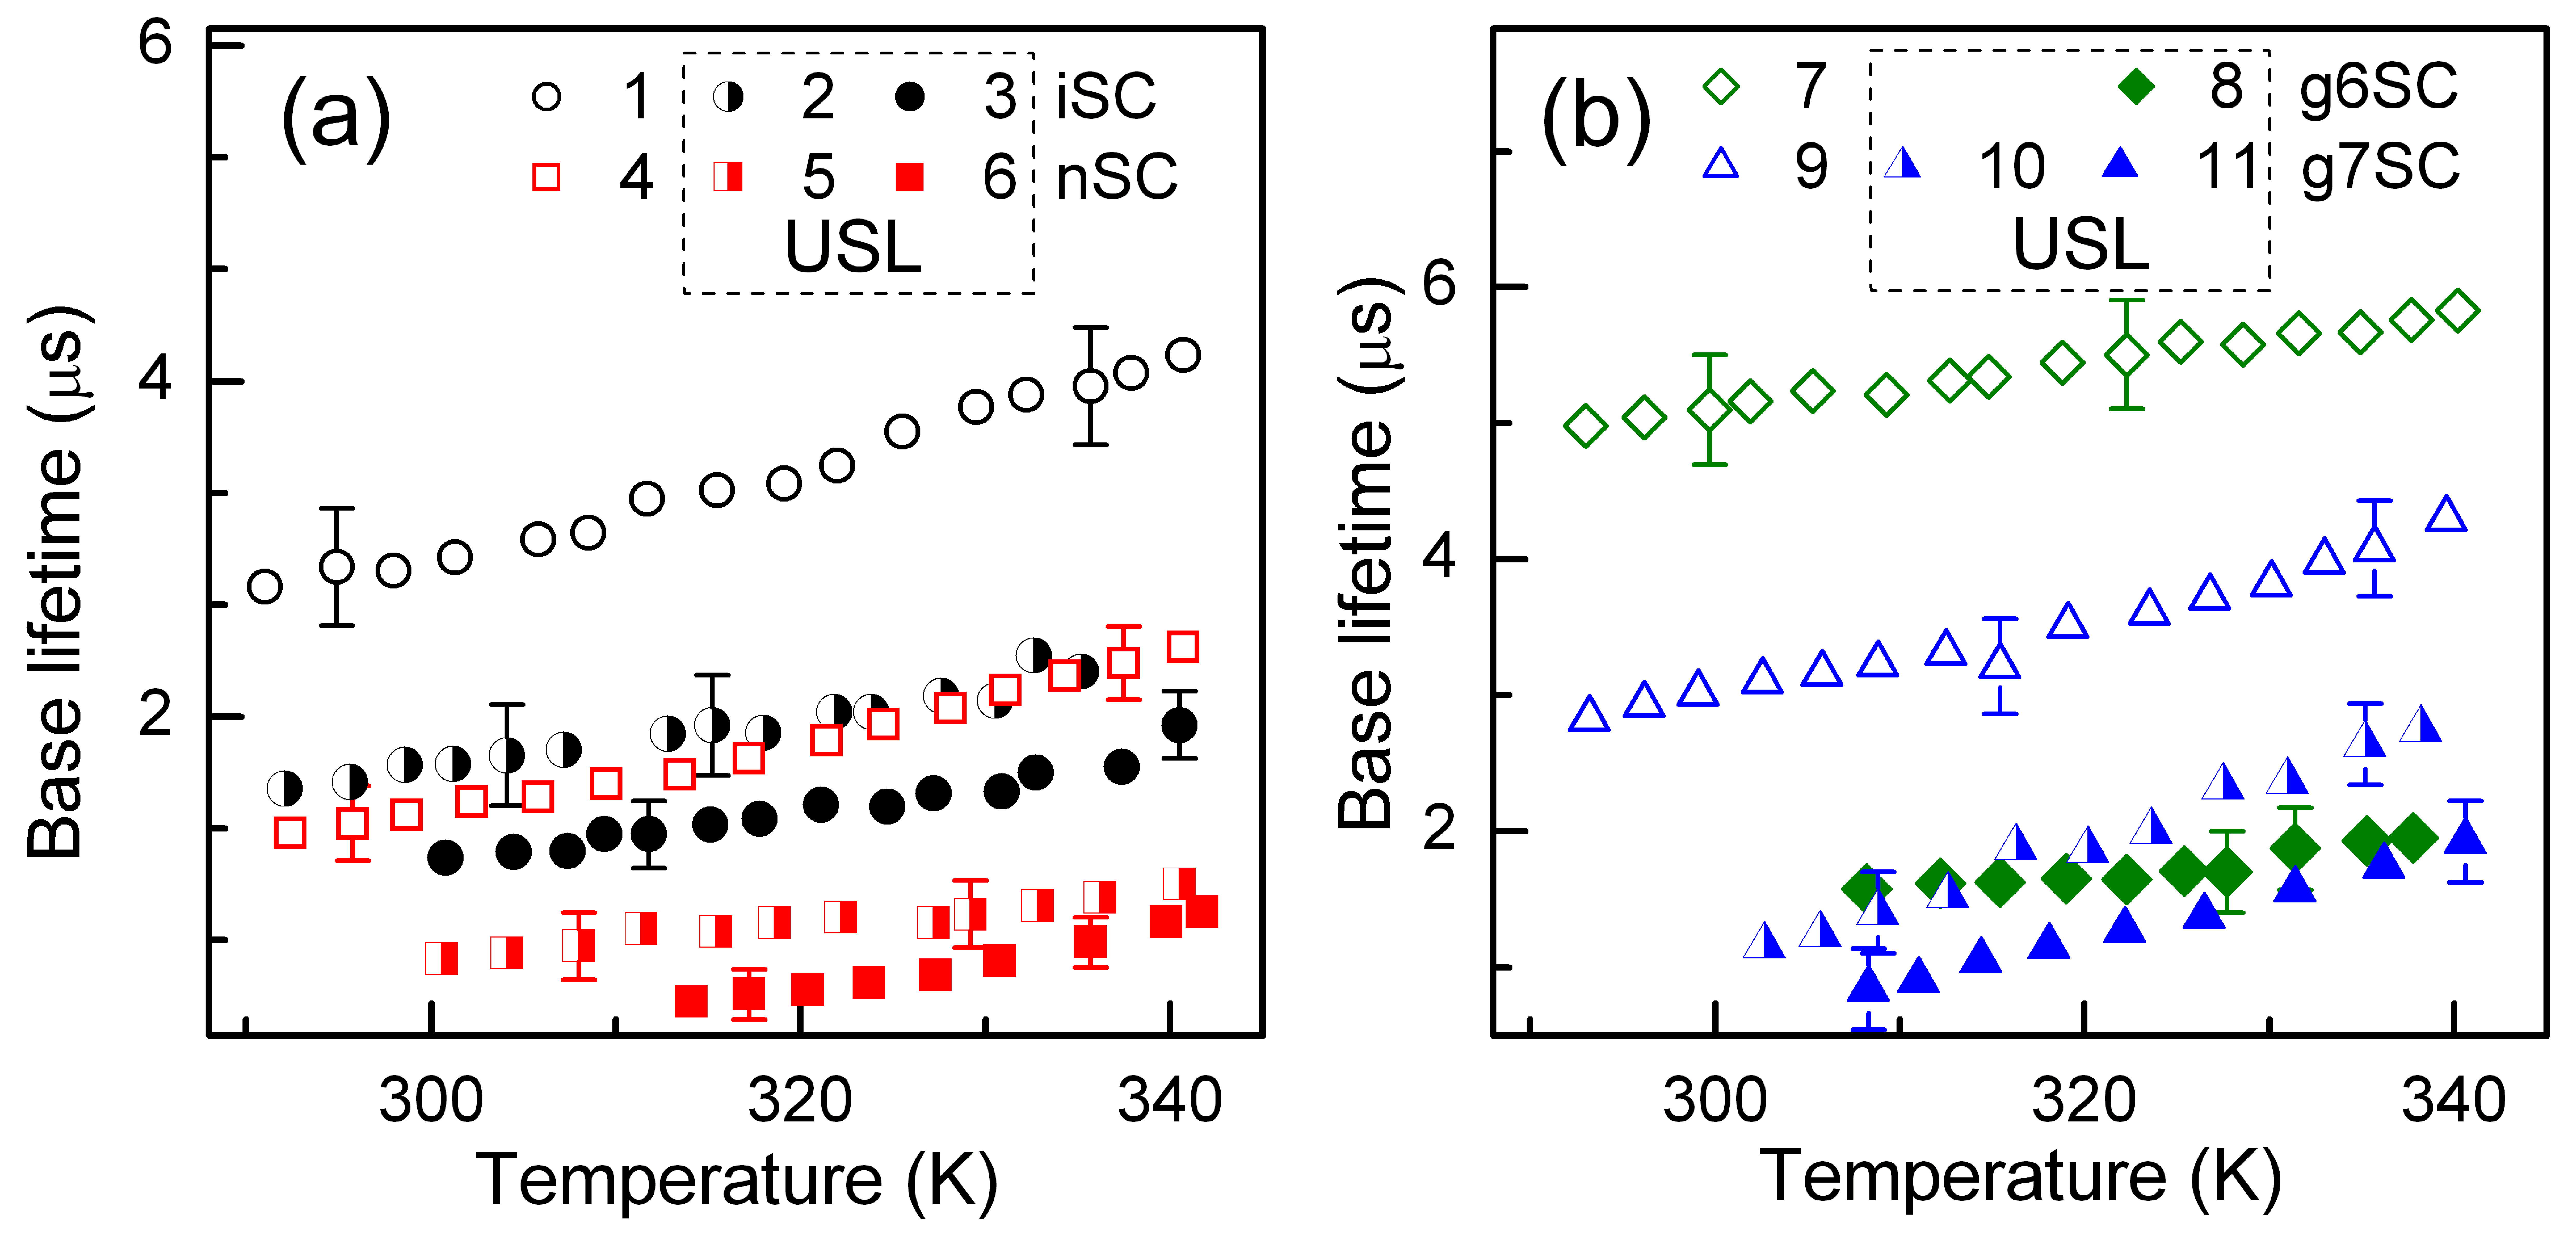
\includegraphics[width=0.7\textwidth]{olikhFig6}%
\caption{\label{fig_TAUr}
Temperature dependences of base lifetime for non--irradiated (curves 1--3, circles),
neutron--irradiated (4--6, squares) and $\gamma$--irradiated (7--11, diamonds and triangles) samples.
The curves 1, 4, 7 and 9 (open marks) are obtained without USL,
curves 2, 3, 5, 6, 8, 10, and 11 correspond to
Ui--1, Ui--2, Un--1, Un--2, Ug6--2, Ug7--1, and Ug7--2 respectively.
}%
\end{figure*}

Really, the irradiation induced lifetime reduction is described by the Messenger–-Spratt equation:\cite{Markvart}
\begin{equation}
\label{eqMS}
\tau_n^{-1}=\tau_{n0}^{-1}+K_\tau\Psi\,,
\end{equation}
where $\tau_{n0}$ is the minority carrier lifetime in the non--irradiated sample,
and $K_\tau$ is a lifetime damage--constants.
The known $K_\tau$ values and estimated changes of reciprocal base lifetime $K_\tau\Psi$ are shown in Table~\ref{tabTAUn}.
One can see, that expected radiation--induced $\tau_n^{-1}$ change equals to ($8\div17$), 4, and 29~\% of
the measured value for samples nSC, g6SC, and g7SC respectively, and cannot explain the observed dispersion.
Calculated lifetime changes $K_\tau\Psi$ are in quite good agreement with those, which are expected from RDs production --- see Section~\ref{DefectType}.

\begin{table}
\caption{\label{tabTAUn}Measured and estimated base lifetime parameters.
}
\begin{ruledtabular}
\begin{tabular}{ccccc}
%\multirow{2}{*}{Sample} &Irradiation&$D$&$\Psi$ &NIEL (Ref.~\onlinecite{NIEL:Akkerman})& $\Psi$ $\times$NIEL  \\
\multirow{2}{*}{Sample} &$\tau_{n,in}^{-1}$ (320~K)&$K_\tau$&$K_\tau\times\Psi$ &$K_\mathtt{US}^\mathtt{eff}$ \\
%&(10$^5$~s$^{-1}$)&(cm$^2$s$^{-1}$)& (10$^4$~s$^{-1}$)&(cm$^2$W$^{-1}$) \\
&(10$^5$~s$^{-1}$)&(cm$^2/$s)& (10$^4$~s$^{-1}$)&(cm$^2/$W) \\
\hline
iSC&2.9&---&---&3.5\\
%\multirow{2}{*}{nSC}&\multirow{2}{*}{4.7}&10$^{-7}$(Ref.~\onlinecite{NIEL:Jafari})&\multirow{2}{*}{4$\div$8}&\multirow{2}{*}{7.1}\\
nSC&4.7&10$^{-7}$(Ref.~\onlinecite{NIEL:Jafari})&\multirow{2}{*}{4$\div$8}&7.1\\
&&2$\cdot$10$^{-7}$(Ref.~\onlinecite{n:Gaubas})&&\\
g6SC&1.8&5$\cdot$10$^{-12}$&0.8&6.0\\
g7SC&2.8&(Refs.~\onlinecite{NIEL:Jafari}, \onlinecite{gamma:Kolkov})&8&5.2\\
\end{tabular}
\end{ruledtabular}
\end{table}

Base lifetime can be expressed as following:\cite{MurphyJAP2011}
\begin{equation}
\label{eqTAUsum}
\tau_n^{-1}=\tau_\mathtt{bb}^{-1}+\tau_\mathtt{CE\,Auger}^{-1}+\tau_\mathtt{SRH}^{-1}\,,
\end{equation}
where
$\tau_\mathtt{bb}$, $\tau_\mathtt{CE\,Auger}$, $\tau_\mathtt{SRH}$ are the lifetime due to band--to--band, Coloumb--enhanced Auger, and
SRH recombination, respectively.
%In our case, $\tau_\mathtt{bb}^{-1}=14$~s$^-1$, $\tau_\mathtt{CE\,Auger}=6$~s$^-1$.
Calculation shows, that $\tau_\mathtt{bb}^{-1}=14$~s$^{-1}$, $\tau_\mathtt{CE\,Auger}^{-1}=6$~s$^{-1}$,
%therefore $\tau_n=\tau_\mathtt{SRH}$.
therefore $\tau_\mathtt{SRH}$ should be under consideration only.
In the cases of low injection level and single recombination centre, SRH lifetime is described by Eq.~(\ref{eqTAU}).
If several centers are present, then
\begin{equation}
\label{eqTAUSHRsum}
\tau_n^{-1}=\sum_i^{M_d}\tau_{n,i}^{-1}=\sum_i^{M_d}N_{d,i},\sigma_{n,i}\,\upsilon_{\mathrm{th},n}\,,
\end{equation}
where
$M_d$ is total number of center,
$\tau_{n,i}$ characterizes lifetime due to recombination by $i$--th defect,
$N_{d,i}$ and $\sigma_{n,i}$ are concentration and electron CCS of $i$--th defect, recpectivelly.

Fig.~\ref{fig_TAUr} shows, that USL results in $\tau_n$ decrease.
Relative AI changes of reciprocal base lifetime $\varepsilon_{\tau r}=(\tau_{n,in}-\tau_{n,\mathtt{US}})/\tau_{n,\mathtt{US}}$
are listed in Table~\ref{tabAIchange}.
As AI changes is reversible, in our opinion, this effect deals with increase of $\sigma_n$ under US action.
Following the empirical relation  proposed by Ref.~\onlinecite{CDLR:R2}, we assume that Eq.~(\ref{eqSigma})
is correct for complex point defect too.
But in this case, $r$ is the distance between complex component.
According to suggested in Section~\ref{SCR} model, USL leads to $r$ variation
and $\sigma_n$ change in line with Eq.~(\ref{eqEpsSig}).
In case of CDLR, AI change of donor (or/and acceptor) SSC is supplemental to variation of
both coupling parameter and couple distance.
But this effect is a single for base lifetime.

On the other hand, every defect does not take part in AID effectively.
If  $M_d^\mathtt{AA}$ and $M_d^\mathtt{nonAA}$ are total numbers of acoustically active (AA) and non--AA center,
then using Eq~(\ref{eqTAUSHRsum}) base lifetime in sample without and with USL can be expressed as
\begin{eqnarray}
\tau_{n,in}^{-1}&=&\sum_j^{M_d^\mathtt{AA}}N_{d,j},\sigma_{n,j}^{in}\,\upsilon_{\mathrm{th},n}+
\sum_l^{M_d^\mathtt{nonAA}}N_{d,l},\sigma_{n,l}\,\upsilon_{\mathrm{th},n}\,,\nonumber\\
\tau_{n,\mathtt{US}}^{-1}&=&\sum_j^{M_d^\mathtt{AA}}N_{d,j},\sigma_{n,j}^\mathtt{US}\,\upsilon_{\mathrm{th},n}+
\sum_l^{M_d^\mathtt{nonAA}}N_{d,l},\sigma_{n,l}\,\upsilon_{\mathrm{th},n}\,.\nonumber
\end{eqnarray}
Using Eq~(\ref{eqEpsSig}), $\varepsilon_{\tau r}$  results in
\begin{equation}
\label{eqEpsTAU}
\varepsilon_{\tau r}=K_\mathtt{US}^\mathtt{eff}W_\mathtt{US}\,,
\end{equation}
where $K_\mathtt{US}^\mathtt{eff}$ characterizes ADI in the sample
and depends on concentration of both AA and non--AA centers
\begin{equation}
\label{eqKeff}
K_\mathtt{US}^\mathtt{eff}=\sum_j^{M_d^\mathtt{AA}}\frac{\tau_{n,in}}{\tau_{n,j,in}}K_\mathtt{US,j}\,,
\end{equation}
$K_\mathtt{US,j}$ deals with $j$--th defect--ultrasound interaction.

The obtained dependences $\varepsilon_{\tau r}$ vs $W_\mathtt{US}$ are shown in Fig.~\ref{fig_Kus}.
Dependences linearity is evidence of our assumption correctness.
The determined $K_\mathtt{US}^\mathtt{eff}$ values are listed in Table~\ref{tabTAUn}.
The non--monotonic $K_\mathtt{US}^\mathtt{eff}$ alteration with $\gamma$ dose
%may be witness of non--AA of gamma-induced defects and
is under consideration in Section \ref{DefectType}.
% in detail.

\begin{figure}
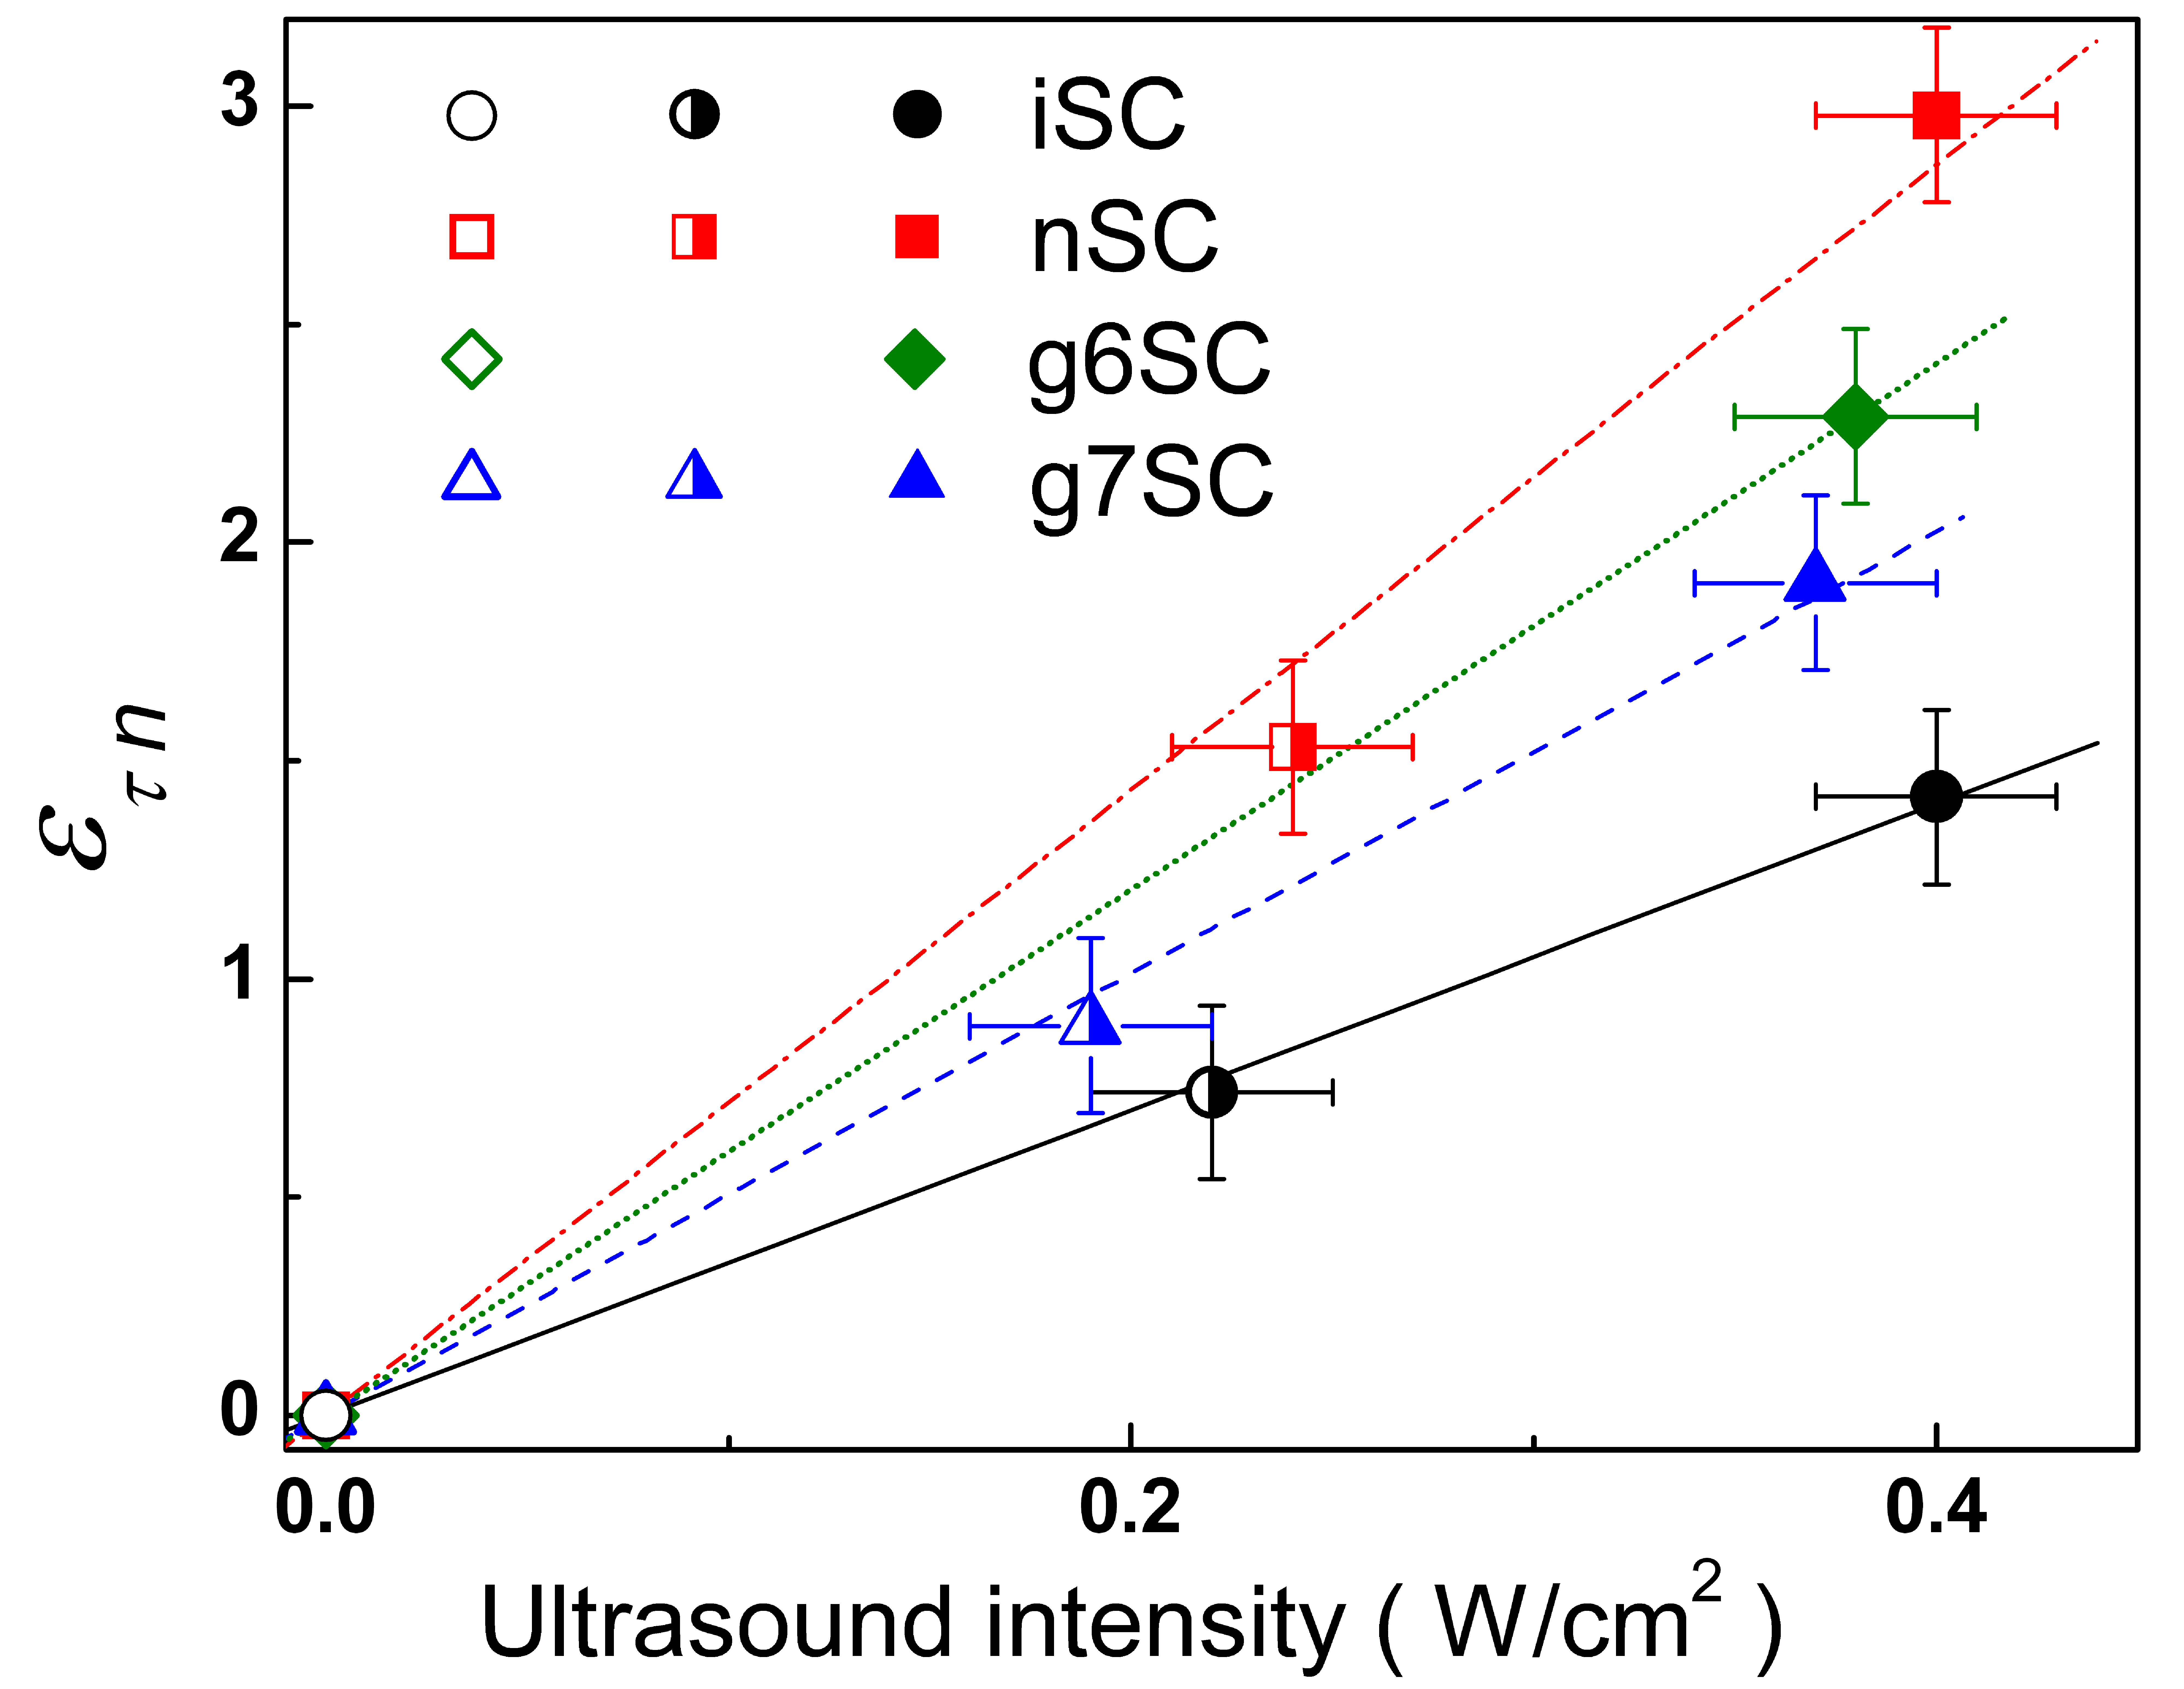
\includegraphics[width=0.45\textwidth]{olikhFig7}%
\caption{\label{fig_Kus}
Dependences of relative base lifetime change on US intensity for non--irradiated (circles), neutron--irradiated (squares), and $\gamma$--irradiated
(triangles and diamonds) samples.
Lines are the fitted curves using Eq.~(\ref{eqEpsTAU}).
}%
\end{figure}

\subsection{Shunt resistance\label{Rsh}}
Fig.~\ref{fig_Rsh} shows the  shunt resistance  over the explored temperature range.
One can see, that irradiation results in $R_{sh}$ decrease.
Besides the $R_{sh}$ temperature dependence behavior is changed in $\gamma$--exposed samples.
Namely the shunt resistance decreases with the temperature growth in iSC and nSC,
whereas close to linear increase of $R_{sh}$ vs $T$  is observed in g6SC and g7SC at 293~K neighbourhood.
We want to notice that $R_{sh}$ axis is logarithmic and linear in Fig.~\ref{fig_Rsh}(a) and Fig.~\ref{fig_Rsh}(b), respectively.

\begin{figure*}
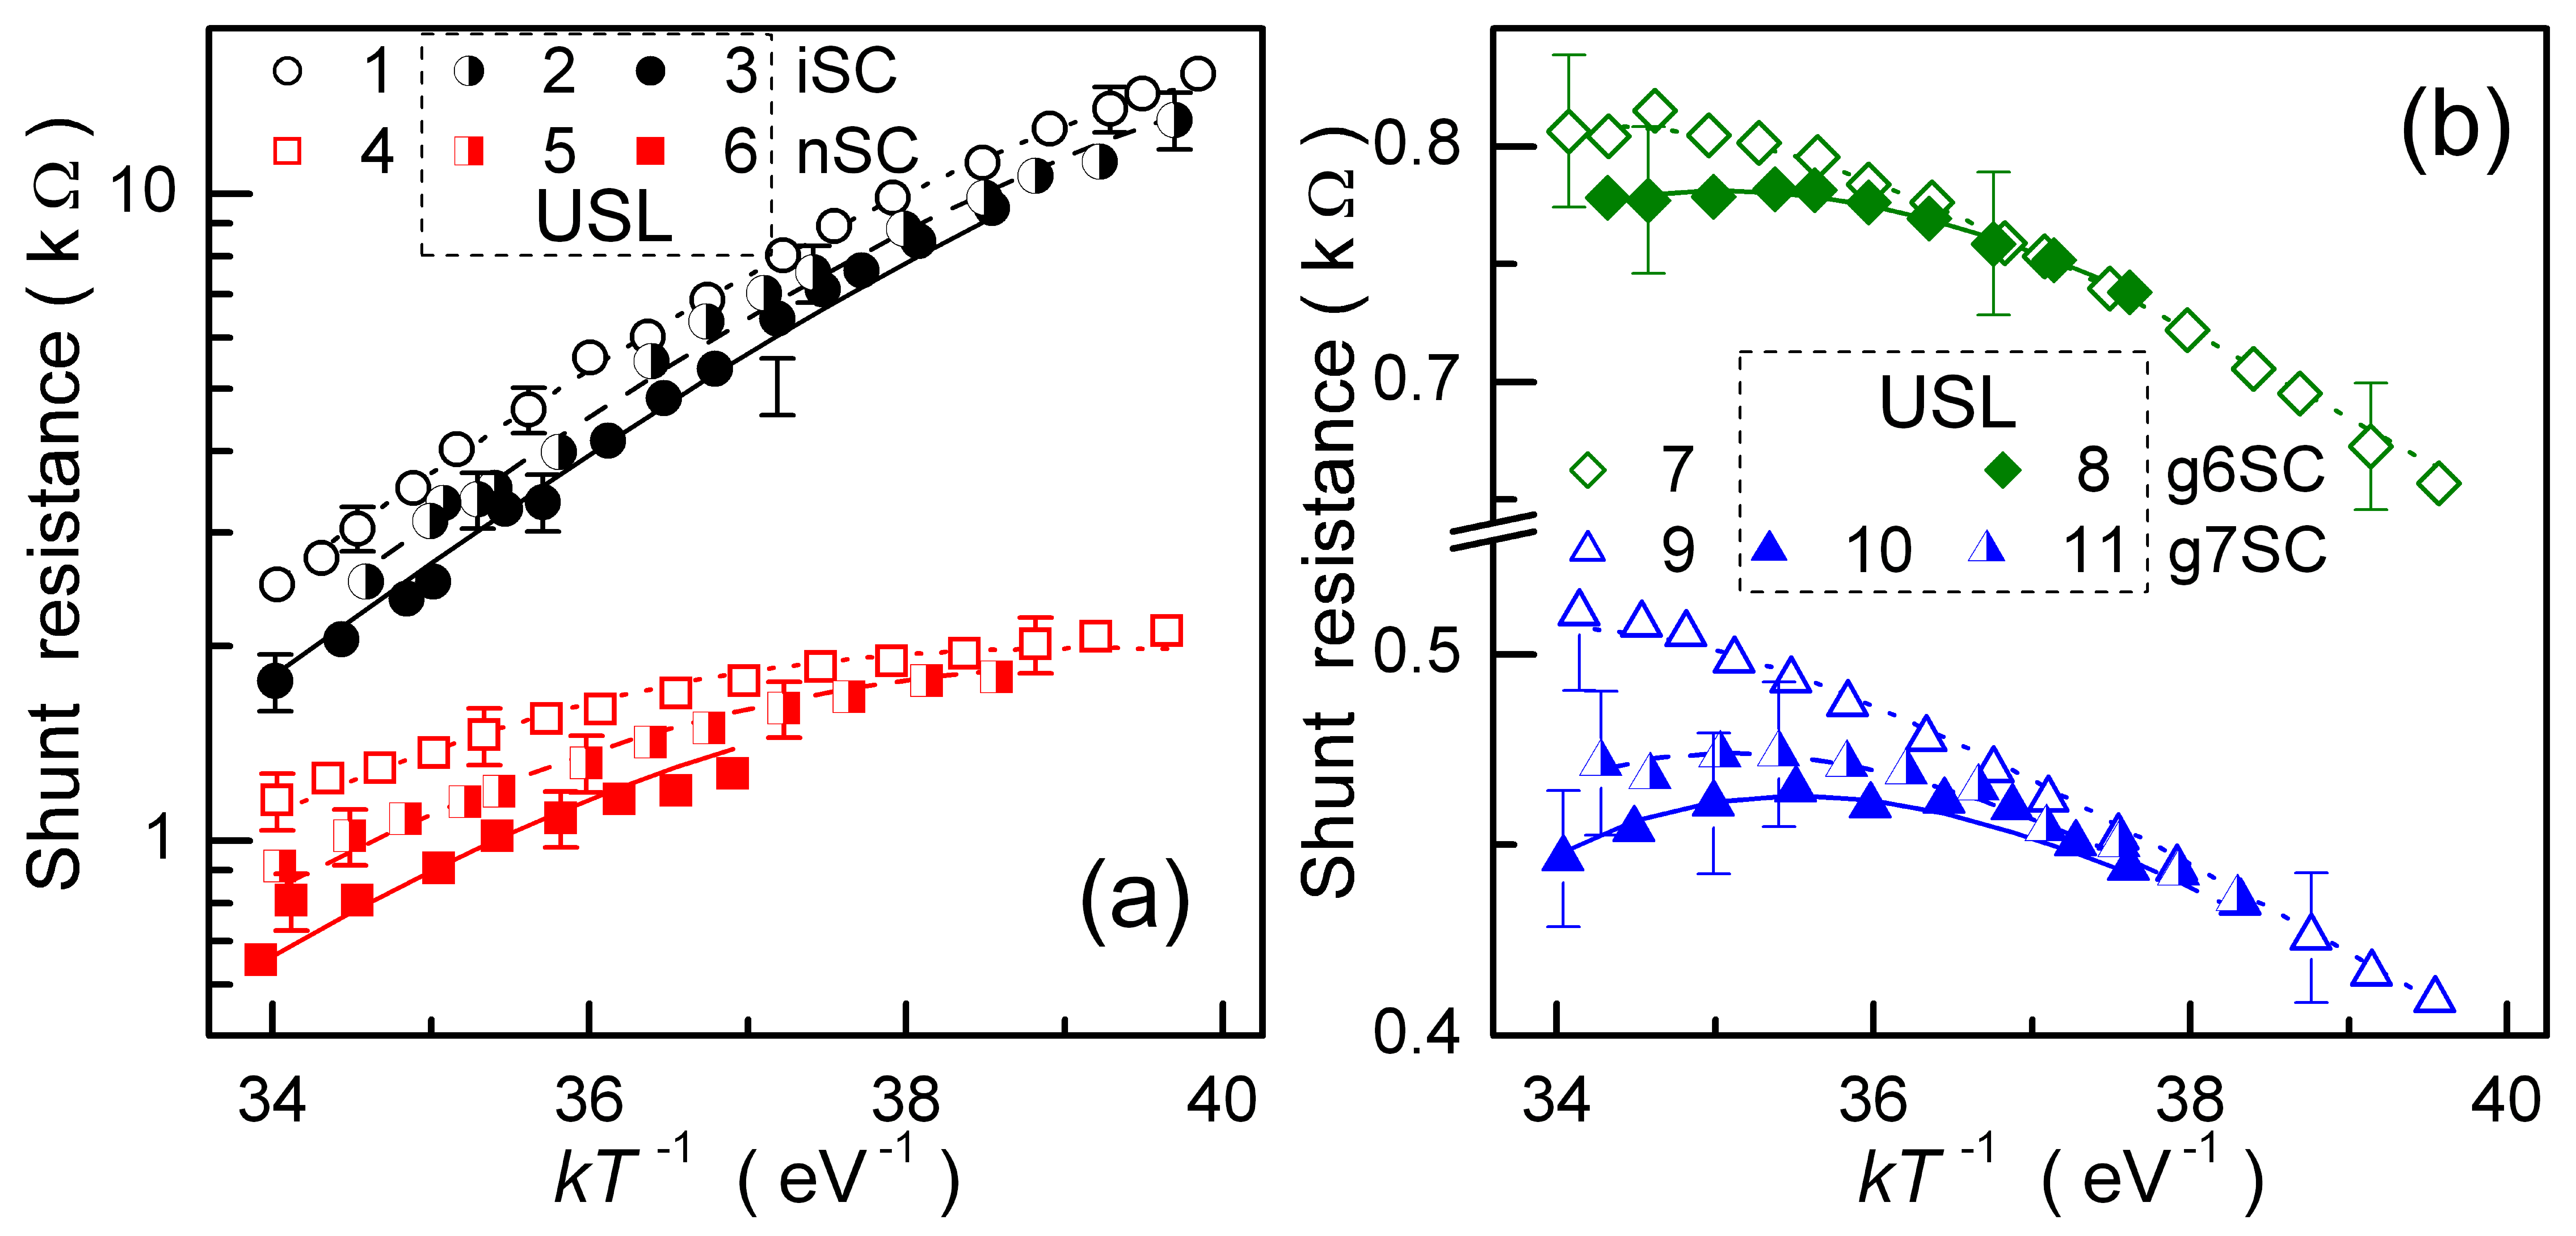
\includegraphics[width=0.7\textwidth]{olikhFig8}%
\caption{\label{fig_Rsh}
Temperature dependences of shunt resistance for non--irradiated (curves 1--3, circles),
neutron--irradiated (4--6, squares) and $\gamma$--irradiated (7--11, diamonds and triangles) samples.
The curves 1, 4, 7 and 9 (open marks) are obtained without USL,
curves 2, 3, 5, 6, 8, 10, and 11 correspond to
Ui--1, Ui--2, Un--1, Un--2, Ug6--2, Ug7--1, and Ug7--2 respectively.
The marks are the experimental results, the lines are the fitted curves using Eq.~(\ref{eqRshFull})-(\ref{eqRsh}).
}%
\end{figure*}

Several non-mechanical reasons of $p$--$n$ structure shunt resistance appearance are known.\cite{Rsh:Breitenstein}
They are aluminum particles, macroscopic Si$_3$N$_4$ inclusions, inversion layers at precipitates.
So during firing Al will alloy in, leading to a $p^+$--doped region around the particle, which may compensate the emitter and may be in ohmic contact with the
base.
Inversion layers and Si$_3$N$_4$ inclusions occur in multicrystalline silicon cells mainly \cite{Rsh:Breitenstein} and cannot cause a shunt resistance of investigated samples.
In addition, dislocations, which intersect the junction, are generally held responsible as a possible source of ohmic current.\cite{Rsh:Breitenstein,TAT:Gopal,Rsh:Baker}
%Dislocations should be strongly recombinative, its recombination current may become strong enough for it to act as a shunt.
In our opinion, both aluminum particles and dislocations are present in the investigated structure.
The overall shunt resistance can be expressed as
\begin{equation}
\label{eqRshFull}
R_{sh}^{-1}=R_{sh,\mathtt{Al}}^{-1}+R_{sh,\mathtt{dis}}^{-1}\,,
\end{equation}
where
$R_{sh,\mathtt{Al}}$ and $R_{sh,\mathtt{dis}}$ deal with aluminum particles and dislocations, respectively.
The linear temperature dependence of metal particles $R_{sh,\mathtt{Al}}$ is suggested:
\begin{equation}
\label{eqRshAl}
R_{sh,\mathtt{Al}}=R_{293,\mathtt{Al}}[1+\alpha(T-293)]\,,
\end{equation}
where
$R_{293,\mathtt{Al}}$ is the shunt resistance at 293~K and
$\alpha$ is the resistance temperature coefficient.

Gopal and Gupta \cite{Rsh:Gopal2003,Rsh:Gopal2004} introduced the model of dislocation--induced impedance of photovoltaic detector.
According to this model, the $R_{sh,\mathtt{dis}}$ can be given by
\begin{equation}
\label{eqRsh}
R_{sh,\mathtt{dis}}=\frac{T}{\sigma_{\mathtt{dis}}}\left[\cosh\left(\frac{E_\mathtt{dis}-E_i}{kT}\right)+\cosh\left(\frac{U_s}{kT}\right)\right]\,,
\end{equation}
with
\begin{equation}
\label{eqRdis}
%\sigma_{\mathtt{dis}}=\rho_{\mathtt{dis}}Aq^2A_{\mathtt{dis}}\sqrt{K_nK_p}\,N_{\mathtt{dis}}(n_p+p_p)k^{-1}\,,
\sigma_{\mathtt{dis}}=\rho_{\mathtt{dis}}Aq^2A_{\mathtt{dis}}\sqrt{K_nK_p}\,N_{\mathtt{dis}}(n_p+p_p)/k\,,
\end{equation}
where
$E_{\mathtt{dis}}$ is the energy level which significantly contributes to the dislocation recombination current,
$U_s$ is the potential at the surface of the dislocation core,
$\rho_{\mathtt{dis}}$ and $A_{\mathtt{dis}}$ are the dislocation density and surface area, respectively,
$K_n$ and $K_p$ are the capture probabilities for electrons and holes by the dislocation states,
$N_{\mathtt{dis}}$ is the density of surface states at each dislocation.
Eq.~(\ref{eqRsh}) is reduced for the simplified case of $K_p=K_n$.

$\alpha$ was determined from g7SC data.
Obtained value $8.3\cdot10^{-3}$~K$^{-1}$ is not far from resistance temperature coefficient of bulk Al ($4.3\cdot10^{-3}$~K$^{-1}$).
Then we used Eqs.~(\ref{eqRshFull})--(\ref{eqRsh}) to fit the experimental $R_{sh}$ data.
$R_{293,\mathtt{Al}}$, $(E_{\mathtt{dis}}-E_i)$, $U_s$, and $\sigma_{\mathtt{dis}}$ were taken as the fitting parameters.
It was established that the good agreement of the experimental data with the fitting curves has been observed (see Fig.~\ref{fig_Rsh}) for values $(E_{\mathtt{dis}}-E_i)=(0.46\pm0.02)$~eV and $U_s=(5\pm4)\times10^{-8}$~eV, which were independent of irradiation and USL.
The obtained $(E_{\mathtt{dis}}-E_i)$ corresponds to the carrier activation energy $0.10\pm0.02$~eV.
This value is comparable to the
activation energy of dislocation levels $0.08$~eV,
which was early reported\cite{disl10:Castaldini,disl10:Isakova,disl10:Yu,disl10:Kveder,disl10:Trushin}
in Cz--Si:B too.\cite{disl10:Castaldini,disl10:Isakova,disl10:Yu}
%early reported \cite{disl10:Castaldini,disl10:Isakova,disl10:Yu,disl10:Kveder,disl10:Trushin}
%value $0.08$~eV, which is associated with dislocation levels, in particular, in Czochralski grown B--doped Si \cite{disl10:Castaldini,disl10:Isakova,disl10:Yu}.



Obtained $R_{293,\mathtt{Al}}$ and $\sigma_{\mathtt{dis}}$ are listed in Table~\ref{tabTpar}.
$R_{293,\mathtt{Al}}$ does not depend on USL and increases with irradiation level.
In our opinion, $R_{sh,\mathtt{dis}}$ is less than $R_{sh,\mathtt{Al}}$ in iSC.
Irradiation leads to vacancy production and Al diffusion out of electrodes.
As a result, Al particle quantity rises, $R_{sh,\mathtt{Al}}$ decreases and becomes key of overall shunt resistance value.
The Al diffusion is more effective in $\gamma$--exposed samples due to more uniform distribution of irradiation--induced single vacancies.

%are in quite good agreement with
$\sigma_{\mathtt{dis}}$ dispersion on sample set correlates to $\tau_n$ that.
Hence it deals with wafer inhomogeneity too.
USL leads to $\sigma_{\mathtt{dis}}$ increase, relative AI changes
$\varepsilon_{\sigma\mathtt{dis}}=(\sigma_{\mathtt{dis,US}}-\sigma_{\mathtt{dis},in})/\sigma_{\mathtt{dis},in}$
are shown in Table~\ref{tabAIchange}.
On our opinion this is caused by an $A_\mathtt{dis}$ augmentation.
Namely, the dislocation core atom displacement  is  normal to the  current direction.
As the result, carriers are captured by dislocation levels from enlarged volume.
Therefore the effective surface area increases and L$R_{sh,\mathtt{dis}}$ decreases under US action.


\subsection{Defect type speculation\label{DefectType}}

Lifetime killers  in boron--doped Czochralski--grown Si are the  boron--oxygen related (BO) defects,\cite{LIDRev,LIDRev2}
iron--boron pairs \cite{MurphyJAP2011,FeB:Vahanissi,FeB:Schmidt} (or another Fe--related trap in the $n^+p$--junctions \cite{TeimurazPSS,TeimurazJAP}),
and oxide precipitates.\cite{MurphySC2014,Oxide_Schon,MurphyJAP2011,MurphyJAP2012,Oxide:Chen,Oxide:Porrini}
The first two defects are sensitive to an intensive illumination at room temperature.
To determine the major recombination center of investigated samples the following experimental procedure has been used.
The non-irradiated sample was light soaked under halogen lamp (2 Suns) illumination at approximately 305~K.
The illumination varied from 1~h to 8~h.
After illumination sample is stored in the dark at room temperature.
To determine the parameters kinetics $I$--$V$ characteristics have been measured with interval 10--15~min at room temperature over a period 5~h after illumination stopping.
To determine the permanent light--induced change the $I$--$V$ characteristics have been measured in 48~h after illumination.
After accumulated time under illumination had run up to 15~h the iSC was annealed at 200~$^\circ$C for $10$~min in the dark and parameters were determined at room temperature.
After that, the illumination and measurements were repeated.

In order to keep the volume of this paper at an rather reasonable size, the detailed results are not shown.
But main result are following.
Illumination did not result in permanent change of either of $\tau_g$, $\tau_n$, $n_{\mathrm{id}}$ before as well as after annealing.
Therefore BO influence on recombination in both SCR and base can be neglected.
$n_{\mathrm{id}}$ increase (about 0.03) and $\tau_g$ decrease (about 10~\%) were observed after illumination immediately.
These changes vanished gradually, both $n_{\mathrm{id}}$ and $\tau_g$ time dependences were very similar to those, which is expected \cite{FeB:Schmidt} for Fe$_i$B$_s$ repairing.
Hence iron--boron pairs take part in SCR recombination.
On the other hand, electron and hole CCS of released by illumination interstitial iron are 1.7 and 0.04 times \cite{FeB:Schmidt} as much as those of Fe$_i$B$_s$.
A small (about 10~\%) $\tau_g$ alteration, which is caused by light, is evidence of supporting role of iron--boron pair in SCR recombination.
Furthermore, since $\tau_n$ does not depend on illumination, then Fe$_i$B$_s$ has not an influence on base lifetime.

As a result, oxide precipitates are number one in SCR and base recombination.
According to Murphy \emph{et al}.\cite{MurphySC2014,MurphyJAP2012},
at least two independent oxide precipitate related defects are exist.
These defects have $\sigma_n/\sigma_p=157$ and $\sigma_p/\sigma_n=1200$ respectively.\cite{MurphyJAP2012}
So, they are suitable to CDLR.
On the basis of mentioned above, we conclude that the defect, which responsible for AI phenomena in nSC, is oxide precipitate mainly.

It is worth keeping doping level, oxygen concentration and dose in mind when RD type is foreseen.
In our case (Czochralski, oxygen--rich, $\sim7\cdot10^{17}$~cm$^{-3}$, $p$--Si with boron concentration $\sim10^{15}$~cm$^{-3}$ and low dose)
it is expected, that C$_i$O$_i$, vacancy clusters V$_n$ (divacancy V$_2$, trivacancy V$_3$, ...) and VO$_i$
are produced mainly by neutron irradiation \cite{n:long,n:gamma,Moll:PhD}
and C$_i$O$_i$ and  VO$_i$ by $\gamma$--rays.\cite{gamma:Stahl,Moll:PhD,gamma:Kolk,A:Caracas}
The RD concentration $N_{t,\mathtt{RD}}$ is proportionate to dose,
the known introduction rate for neutron $\eta_n$ and gamma $\eta_\gamma$ irradiation in Cz--Si are shown in Table~\ref{tabDefect}.
The expected $N_{t,\mathtt{RD}}$ for investigated samples are listed in Table~\ref{tabDefect} too.

%\begin{table}
%\caption{\label{tabDefect}Used defect parameters.
%}
%\begin{ruledtabular}
%\begin{tabular}{cccc}
%Defect&$\sigma_n$&$\eta_n$ (cm$^{-1}$)&$\eta_\gamma$\\
%&(10$^{-15}$~cm$^2$)&Ref.~\onlinecite{Moll:PhD}&\\
%\hline
%C$_i$O$_i$&0.7 (Ref.~\onlinecite{gamma:Stahl})&1.38&6$\cdot$10$^5$~rad$^{-1}$cm$^{-3}$ (Ref.~\onlinecite{gamma:Stahl})\\
%&0.9 (Ref.~\onlinecite{gamma:Kolk})&&4$\cdot$10$^{-4}$~cm$^{-1}$ (Ref.~\onlinecite{gamma:Kolk})\\
%V$_2$&3 (Ref.~\onlinecite{gamma:Stahl})&1.21&3$\cdot$10$^4$~rad$^{-1}$cm$^{-3}$ (Ref.~\onlinecite{gamma:Stahl})\\
%&2 (Ref.~\onlinecite{A:Brothe})&&\\
%V$_3$&2.4 (Ref.~\onlinecite{V3:Markevich})&0.37&---\\
%VO$_i$&2.4 (Ref.~\onlinecite{A:Caracas})&0.52&7$\cdot$10$^5$~rad$^{-1}$cm$^{-3}$ (Ref.~\onlinecite{gamma:Stahl})\\
%&4 (Ref.~\onlinecite{A:Bleicher})&&4$\cdot$10$^{-4}$~cm$^{-1}$ (Ref.~\onlinecite{gamma:Kolk})
%\end{tabular}
%\end{ruledtabular}
%\end{table}



\begin{table*}
\caption{\label{tabDefect}Cited and calculated defect parameters.
}
\begin{ruledtabular}
\begin{tabular}{cccccccccc}
Defect&$\sigma_n$&$\eta_n$ (cm$^{-1}$)&$\eta_\gamma$&\multicolumn{3}{c}{$N_{t,\mathtt{RD}}$(10$^{11}$~cm$^{-3}$)}&\multicolumn{3}{c}{$\tau_{n,\mathtt{RD}}^{-1}$ (10$^4$~s$^{-1}$)}\\
&(10$^{-15}$~cm$^2$)&Ref.~\onlinecite{Moll:PhD}&&nSC&g6SC&g7SC&nSC&g6SC&g7SC\\
\hline
C$_i$O$_i$&0.7 (Ref.~\onlinecite{gamma:Stahl})&1.38&6$\cdot$10$^5$~rad$^{-1}$cm$^{-3}$ (Ref.~\onlinecite{gamma:Stahl})&5.5&6&60&$0.8\div1$&$0.9\div1.1$&$9\div11$\\
&0.9 (Ref.~\onlinecite{gamma:Kolk})&&4$\cdot$10$^{-4}$~cm$^{-1}$ (Ref.~\onlinecite{gamma:Kolk})&&&&&&\\
V$_2$&3 (Ref.~\onlinecite{gamma:Stahl})&1.21&3$\cdot$10$^4$~rad$^{-1}$cm$^{-3}$ (Ref.~\onlinecite{gamma:Stahl})&4.8&0.3&3&$2.2\div3.3$&$0.1\div0.2$&$1\div2$\\
&2 (Ref.~\onlinecite{A:Brothe})&&&&&&&&\\
V$_3$&2.4 (Ref.~\onlinecite{V3:Markevich})&0.37&---&1.5&---&---&0.7&---&---\\
VO$_i$&2.4 (Ref.~\onlinecite{A:Caracas})&0.52&7$\cdot$10$^5$~rad$^{-1}$cm$^{-3}$ (Ref.~\onlinecite{gamma:Stahl})&2&$6\div7$&$60\div70$&&&\\
&4 (Ref.~\onlinecite{A:Bleicher})&&4$\cdot$10$^{-4}$~cm$^{-1}$ (Ref.~\onlinecite{gamma:Kolk})&&&&&&
\end{tabular}
\end{ruledtabular}
\end{table*}


%\begin{table*}
%\caption{\label{tabIrrad}Estimated RD concentrations and their influence on reciprocal base lifetime.
%}
%\begin{ruledtabular}
%\begin{tabular}{cccccccc}
%\multirow{2}{*}{Sample}&\multicolumn{4}{c}{$N_{t,\mathtt{RD}}$ (10$^{11}$~cm$^{-3}$)}&\multicolumn{3}{c}{$\tau_{n,\mathtt{RD}}^{-1}$ (10$^4$~s$^{-1}$)}\\
%& C$_i$O$_i$ & V$_2$ & V$_3$ & VO$_i$ & C$_i$O$_i$ & V$_2$ & V$_3$ \\
%\hline
%nSC&5.5&4.8&1.5&2&$0.8\div1$&$2.2\div3.3$&0.7\\
%g6SC&6&0.3&0&$6\div7$&$0.9\div1.1$&$0.1\div0.2$&0\\
%g7SC&60&3&0&$60\div70$&$9\div11$&$1\div2$&0\\
%\end{tabular}
%\end{ruledtabular}
%\end{table*}

Another defects, which can be created by irradiation in silicon, are I$_p$--center, bistable donor (BD), B$_i$O$_i$ and C$_i$C$_s$.
But first and second defects are characterized by small introduction rate.
For example, BD expected\cite{n:gamma,BD:Fret} concentration is only $(1\div2)\cdot10^{10}$~cm$^{-3}$ in nSC and g7SC.
B$_i$O$_i$ lack in investigated samples deals with low boron concentration \cite{SiIntDef}.
Lastly,  C$_i$C$_s$ creation is suppressed in oxygen--rich crystal.\cite{gamma:Kolk,gamma:Stahl,n:long}
Besides C$_i$C$_s$ is not recombination active center.\cite{CiCs:Song}

%Eq.~(\ref{eqTAUSHRsum}) can be used to estimate each RD influence on base lifetime.
To estimate RD influence on base lifetime, one can use Eq.~(\ref{eqTAUSHRsum})
and takes into account, that
VO$_i$ is not active recombination center in $p$--Si.\cite{gamma:Kolkov,IrrCzpSi:Benton,IrrCzpSi:Coffa,IrrCzpSi:Ganagona,IrrCzpSi:Vines}
%Eq.~(\ref{eqTAUSHRsum}) show that, each RD separate influence on $\tau_n$ is connected with $\tau_{n,\mathtt{RD}}$ of individual defect.
%$\tau_{n,\mathtt{RD}}$ are calculated by using Eq.~(\ref{eqTAU}) and are listed in Table~\ref{tabIrrad}.
%It is taking into account, that VO$_i$ is not recombination center in $p$--Si \cite{gamma:Kolkov,IrrCzpSi:Benton,IrrCzpSi:Coffa,IrrCzpSi:Ganagona,IrrCzpSi:Vines}.
Estimated $\tau_{n,\mathtt{RD}}$ for C$_i$O$_i$, V$_2$, and  V$_3$ are shown in Table~\ref{tabDefect}.
One can recognize, that $\tau_n$ effected mainly by C$_i$O$_i$ and vacancy clusters in $\gamma$-- and neutron--irradiated samples, respectively.
We want to note, that nSc, g6Sc, g7SC sums of $\tau_{n,\mathtt{RD}}$ are in quite good agreement with $(K_\tau\cdot\Psi)$ values.

Lets pay attention to $K_\mathtt{US}^\mathtt{eff}$ and assume, that
$M_d^\mathtt{AA}=1$, $M_d^\mathtt{nonAA}=1$ in non--irradiated sample and
US interaction with C$_i$O$_i$ and V$_n$ is described by $K_\mathtt{US}^\mathtt{CO}$ and $K_\mathtt{US}^\mathtt{V}$, respectively.
Using Eq.~(\ref{eqKeff}),
$K_\mathtt{US}^\mathtt{eff}$ for nSC and irradiated samples
can be expressed as
%\begin{equation}
%K_\mathtt{US}^\mathtt{eff}=K_\mathtt{US}^\mathtt{AA}\,\tau_{n,in}/\tau_{n,in}^\mathtt{AA}\,,\nonumber
%\end{equation}
%for nSC and
\begin{eqnarray}
K_\mathtt{US}^\mathtt{eff}&=&K_\mathtt{US}^\mathtt{AA}\,\tau_{n,in}/\tau_{n,in}^\mathtt{AA}\,,\nonumber\\
K_\mathtt{US}^\mathtt{eff}&=&K_\mathtt{US}^\mathtt{AA}\tau_{n,in}/\tau_{n,in}^\mathtt{AA}+
                           K_\mathtt{US}^\mathtt{CO}\tau_{n,in}/\tau_{n,\mathtt{RD}}^\mathtt{CO}+
                           K_\mathtt{US}^\mathtt{V}\tau_{n,in}/\tau_{n,\mathtt{RD}}^\mathtt{V} \,,\nonumber
\end{eqnarray}
where
$\tau_{n,in}^\mathtt{AA}$ is the base lifetime in case of non-radiative AA defect with $K_\mathtt{US}^\mathtt{AA}$ is only present in sample.

%\begin{equation}
%\label{eqKeffff}
%K_\mathtt{US}^\mathtt{eff}=\sum_j^{M_d^\mathtt{AA}}\frac{\tau_{n,in}}{\tau_{n,j,in}}K_\mathtt{US,j}\,,
%\end{equation}

Two extreme cases are opportune to analysis.
In the first one, non--AA defects are distributed uniformly across wafer and
AA defects define a distinction of
$(\tau_{n,in}^{-1}-K_\tau\cdot\Psi)$ value for different samples.
In the second one, a non--AA defect distribution is not uniform,
whereas $\tau_{n,in}^\mathtt{AA}$ is identical for iSC, nSC, g6SC, and g7SC.
However, in the first case (as well as in case of $M_d^\mathtt{nonAA}=0$),
experimental $K_\mathtt{US}^\mathtt{eff}$ values lead to unreal (negative) values of $K_\mathtt{US,j}$.
In the second case, using Eq.~(\ref{eqKeff}) and data of Tables~\ref{tabTAUn} and \ref{tabDefect}, the following equation array can be written:
\begin{eqnarray}
\mbox{iSC}:\,\,3.5&=&K_\mathtt{US}^\mathtt{AA}\cdot(\tau_{n,in}^\mathtt{AA})^{-1}\,/2.9\,,\nonumber\\
\mbox{nSC}:\,\,7.1&=&K_\mathtt{US}^\mathtt{AA}\cdot(\tau_{n,in}^\mathtt{AA})^{-1}\,/4.7+0.09\,K_\mathtt{US}^\mathtt{V}+0.02\,K_\mathtt{US}^\mathtt{CO}\,,\nonumber\\
\mbox{g6SC}:\,\,6.0&=&K_\mathtt{US}^\mathtt{AA}\cdot(\tau_{n,in}^\mathtt{AA})^{-1}\,/1.8+0.01\,K_\mathtt{US}^\mathtt{V}+0.05\,K_\mathtt{US}^\mathtt{CO}\,,\nonumber\\
\mbox{g7SC}:\,\,5.2&=&K_\mathtt{US}^\mathtt{AA}\cdot(\tau_{n,in}^\mathtt{AA})^{-1}\,/2.8+0.05\,K_\mathtt{US}^\mathtt{V}+0.35\,K_\mathtt{US}^\mathtt{CO}\,,\nonumber
%\\
%\mbox{iSC}:\,\,3.5&=&K_\mathtt{US}^\mathtt{AA}\,/2.9\,\tau_{n,in}^{\mathtt{AA}}\,,\nonumber\\
%\mbox{nSC}:\,\,7.1&=&K_\mathtt{US}^\mathtt{AA}\,/4.7\,\tau_{n,in}^{\mathtt{AA}}+0.09\,K_\mathtt{US}^\mathtt{V}+0.02\,K_\mathtt{US}^\mathtt{CO}\,,\nonumber\\
%\mbox{g6SC}:\,\,6.0&=&K_\mathtt{US}^\mathtt{AA}\,/1.8\,\tau_{n,in}^{\mathtt{AA}}+0.01\,K_\mathtt{US}^\mathtt{V}+0.05\,K_\mathtt{US}^\mathtt{CO}\,,\nonumber\\
%\mbox{g7SC}:\,\,5.2&=&K_\mathtt{US}^\mathtt{AA}\,/2.8\,\tau_{n,in}^{\mathtt{AA}}+0.05\,K_\mathtt{US}^\mathtt{V}+0.35\,K_\mathtt{US}^\mathtt{CO}\,,\nonumber
\end{eqnarray}
where
$(\tau_{n,in}^\mathtt{AA})^{-1}$ in $10^4$/~s.
These equations are correct if
$K_\mathtt{US}^\mathtt{AA}\cdot(\tau_{n,in}^\mathtt{AA})^{-1}=(10\pm3)$~cm$^2$/W,
$K_\mathtt{US}^\mathtt{V}=(42\pm15)$~cm$^2$/W,
$K_\mathtt{US}^\mathtt{CO}=0$.
Since $(\tau_{n,in}^\mathtt{AA})^{-1}<1.83$, then $K_\mathtt{US}^\mathtt{AA}>5$~cm$^2$/W.
Thus observed base lifetime change is caused by AI modification of the same defect (most likely oxide precipitates) in
both non--irradiated and $\gamma$--irradiated samples.
This effect is added by AI divacancy alteration in neutron--irradiated samples.
In other words, C$_i$O$_i$ is non--AA defect, whereas V$_2$ is AA defect.

As to SCR recombination, in our judgement, $\tau_g$ and $n_\mathrm{id}$ in non--irradiated sample
are affected by modification of coupled oxide precipitate related defects under US action.
As assumed above  in Section \ref{SCR},
the AA radiation defects with $\Delta\Omega_d<0$ take part in CDLR in irradiated samples.
Divacancy is quite suitable for AI influence on $\tau_g$ and $n_\mathrm{id}$ in nSC.
But a bistable (or metastable) defect is expected in $\gamma$--irradiated samples.
There are known a few such defect with $\Delta\Omega_d<0$ in Si,
viz VO$_2$,\cite{V2Obistable}
V$_3$,\cite{V3:Markevich}
and VO$_i$.\cite{Bistable:UFN}
VO$_2$ appears after $300^\circ$C annealing of irradiated crystal,
V$_3$ is not typical defect for $\gamma-^{60}$Co exposed silicon.
On the other hand, VO$_i$ is largo manum produced and can take part in CDLR around $n^+$--$p$
interface in g6SC and g7SC.
Metastable state, which is commonly observed at low temperature, differs by large distance between oxygen and vacancy and
by  more deep energy level.\cite{Bistable:UFN}
The volume change of entire complex is negative,
whereas for complex component $\Delta\Omega_d(\mbox{V})<0$ and
$\Delta\Omega_d(\mbox{O}_i)>0$.
Hence, under assumption, VO$_i$ is favorable pair for AI alteration of component distance.
Thus VO$_i$ can be rebuild to metastable configuration by USL and
this effect results in  both $T_{\mathrm{id}}$ and $E_{\tau g}$ change.



\section{Conclusion}
The experimental investigation of ultrasound influence on the $I$--$V$ characteristic of silicon $n^+$--$p$--structure has been carried out.
The effects of reactor neutrons and $^{60}$Co gamma radiation on ultrasound influence were studied.
The investigation has revealed the acoustically driven reversible decrease of both minority carrier lifetime in structure base and shunt resistance.
The effect intensifies in irradiated structures.
The analysis has shown that the acoustically induced increase of carrier capture coefficient of point or extended defects is a reason of observed effects.
It has been found out that the ultrasound loading leads to the reversible modification of SCR carrier lifetime and ideality factor.
Changes are opposite in sign in non--irradiated and irradiated structures.
The qualitative model of observed phenomenon, which is based on the increase of a distance between coupled defects or between defect complex components under ultrasound action, has been under consideration.
It has been shown that divacancy and pair vacancy--interstitial oxygen are effectively modified by ultrasound in neutron-- and $\gamma$--exposed structures respectively.
Complex interstitial carbon--interstitial oxygen does not practically take part in acousto--defect interaction.
Thus, ultrasound can be an effective tool for controlling silicon structure characteristics.

\bibliography{olikh}



\end{document}

